% -------------------- Result and Analysis ----------------------------------



\section{Test Plans, Results and Analysis}
%Prepare the test plans in tabular format, where each Test Case should be represented with distinct id, prefixed with “$\langle$module$\rangle$ “, where module represents the short code of the respective design module. Test Case numbers should be matching as stated in Requirement Matrix.
%\vspace{.1in}

%\noindent

%Appropriate definition of ‘Performance Metrics’, e.g. Classification Accuracy, Mean Squared Error etc. should be included, as applicable. 
%\vspace{.1in}

%\noindent
%Depending on your specific project, test results can be represented as a table of data with a corresponding pie chart / bar chart as needed. Analysis of test results should be discussed in terms of clear bullet points.

\begin{table}[H]
    \caption*{Test Case Plan Table}
    \centering
    \resizebox{\textwidth}{!}{
    \begin{tabularx}{\textwidth}{|>{\centering\arraybackslash}m{1.5cm}|X|X|X|>{\centering\arraybackslash}m{1.5cm}|}
        \hline
        \textbf{Test Case ID} & \textbf{Description} & \textbf{Expected Result} & \textbf{Actual Result} & \textbf{Status} \\ \hline
        T01 & User provides input in the text area. & Text is accepted for further processing. & Text is accepted for further processing. & \checkmark \\ \hline
        T02 & Display mental health issues with probabilities for classes. & Probabilities for each mental health class are shown. & Probabilities for each mental health class are shown. & \checkmark \\ \hline
        T03 & Highlight the mental health issue with the highest probability. & Correct issue with the highest probability is displayed. & Correct issue with the highest probability is displayed. & \checkmark \\ \hline
        T04 & Accept username input and provide prediction. & Prediction is displayed based on the provided username. & Prediction is displayed based on the provided username. & \checkmark \\ \hline
    \end{tabularx}
    }
\end{table}

\pagebreak

\begin{table}[H]
    \caption*{Test Case Plan Table}
    \centering
    \resizebox{\textwidth}{!}{
    \begin{tabularx}{\textwidth}{|>{\centering\arraybackslash}m{1.5cm}|X|X|X|>{\centering\arraybackslash}m{1.5cm}|}
        \hline
        \textbf{Test Case ID} & \textbf{Description} & \textbf{Expected Result} & \textbf{Actual Result} & \textbf{Status} \\ \hline
        T05 & Translate multiple language inputs to English. & Non-English text is translated correctly to English. & Non-English text is translated correctly to English. & \checkmark \\ \hline
        T06 & Extract text and detect emotion from image. & Extracted text and detected emotions are displayed accurately. & Extracted text and detected emotions are displayed accurately. & \checkmark \\ \hline
        T07 & Pass a prompt to the system and retrieve a valid response. & Correct response is generated based on the prompt. & Correct response is generated based on the prompt. & \checkmark \\ \hline
        T08 & Perform a combined test using multiple inputs. & Predictions for all inputs are displayed correctly. & Predictions for all inputs are displayed correctly. & \checkmark \\ \hline
        T09 & Analyze uploaded audio files and transcribe them into text. & Audio transcription and analysis results are displayed. & Audio transcription and analysis results are displayed. & \checkmark \\ \hline
        T10 & Extract frames, analyze emotions, audio from video. & Frame emotions and audio transcription are displayed. & Frame emotions and audio transcription are displayed. & \checkmark \\ \hline
        T11 & Extract tweets and related media using a Twitter username. & Text and media are extracted and analyzed correctly. & Text and media are extracted and analyzed correctly. & \checkmark \\ \hline
        T12 & Generate captions for uploaded images or video frames. & Captions are generated for images or frames. & Captions are generated for images or frames. & \checkmark \\ \hline
        T13 & Upload a PDF file and analyze its text content. & Extracted text from the PDF is processed and analyzed for mental health cues. & Extracted text from the PDF is processed and analyzed for mental health cues. & \checkmark \\ \hline
        T14 & Capture user response to a displayed image. & User response is captured and correctly classified for emotional analysis. & User response is captured and correctly classified for emotional analysis. & \checkmark \\ \hline
        T15 & Fill out a survey form to update the association matrix. & Survey responses update the association matrix and generate targeted wellbeing insights. & Survey responses update the association matrix and generate targeted wellbeing insights. & \checkmark \\ \hline

        T16 & RAG-based Wellbeing Insights & Synthesizes targeted wellbeing insights by leveraging retrieved context, input prompts, and mental health cues. & Generates refined wellbeing insights using GEMINI-2.0-FLASH based on retrieved data. & \checkmark \\ \hline

    \end{tabularx}
    }
\end{table}

\pagebreak

\begin{table}[H]
    \caption*{Metrics for Evaluation}
    \label{tab:metrics}
    \centering
    \begin{tabularx}{\textwidth}{|p{3cm}|>{\raggedright\arraybackslash}X|}
    \hline
    \textbf{Metric} & \textbf{Definition and Formula} \\ \hline
    Precision & The ratio of correctly predicted positive observations to the total predicted positives.
    \[
    \text{Precision} = \frac{TP}{TP + FP}
    \]
    where \(TP\) = True Positives, \(FP\) = False Positives. \\ \hline
    Recall & The ratio of correctly predicted positive observations to all observations in the actual class.
    \[
    \text{Recall} = \frac{TP}{TP + FN}
    \]
    where \(TP\) = True Positives, \(FN\) = False Negatives. \\ \hline
    F1-Score & The harmonic mean of Precision and Recall.
    \[
    \text{F1-Score} = 2 \times \frac{\text{Precision} \times \text{Recall}}{\text{Precision} + \text{Recall}}
    \] \\ \hline
    Support & The number of actual occurrences of each class in the dataset.
    \[
    \text{Support} = \text{Number of samples in the true class}
    \] \\ \hline
    Confusion Matrix & A matrix used to evaluate classification performance:
    \[
    \begin{bmatrix}
    TP & FP \\
    FN & TN
    \end{bmatrix}
    \]
    where \(TP\) = True Positives, \(FP\) = False Positives, \(FN\) = False Negatives, and \(TN\) = True Negatives. \\ \hline
    \end{tabularx}
\end{table}

\subsection{Results from Base Models}

\begin{center}
    \textbf{Logistic Regression} \\[0.5em]
    \begin{tabular}{|l|c|c|c|c|}
        \hline
        \textbf{Class} & \textbf{Precision} & \textbf{Recall} & \textbf{F1-Score} & \textbf{Support} \\ \hline
        Anxiety        & 0.83               & 0.77            & 0.80              & 379              \\ \hline
        Bipolar        & 0.74               & 0.55            & 0.63              & 384              \\ \hline
        Depression     & 0.76               & 0.76            & 0.76              & 373              \\ \hline
        Normal         & 0.92               & 0.99            & 0.95              & 2183             \\ \hline
        PTSD           & 0.87               & 0.77            & 0.82              & 394              \\ \hline
        \textbf{Accuracy} & \multicolumn{4}{|c|}{87.66\%} \\ \hline
        \textbf{Macro Avg} & 0.82            & 0.77            & 0.79              & 3713             \\ \hline
        \textbf{Weighted Avg} & 0.87         & 0.88            & 0.87              & 3713             \\ \hline
    \end{tabular}
\end{center}

\pagebreak
% --------- naive bayes

\begin{center}
    \textbf{Naive Bayes} \\[0.2em]
    \begin{tabular}{|l|c|c|c|c|}
        \hline
        \textbf{Class} & \textbf{Precision} & \textbf{Recall} & \textbf{F1-Score} & \textbf{Support} \\ \hline
        Anxiety        & 0.70               & 0.73            & 0.72              & 379              \\ \hline
        Bipolar        & 0.83               & 0.45            & 0.58              & 384              \\ \hline
        Depression     & 0.59               & 0.87            & 0.70              & 373              \\ \hline
        Normal         & 0.96               & 0.92            & 0.94              & 2183             \\ \hline
        PTSD           & 0.71               & 0.83            & 0.76              & 394              \\ \hline
        \textbf{Accuracy} & \multicolumn{4}{|c|}{83.63\%} \\ \hline
        \textbf{Macro Avg} & 0.76            & 0.76            & 0.74              & 3713             \\ \hline
        \textbf{Weighted Avg} & 0.85         & 0.84            & 0.84              & 3713             \\ \hline
    \end{tabular}
\end{center}

% -------- svm

\begin{center}
    \textbf{Support Vector Machine} \\[0.2em]
    \begin{tabular}{|l|c|c|c|c|}
        \hline
        \textbf{Class} & \textbf{Precision} & \textbf{Recall} & \textbf{F1-Score} & \textbf{Support} \\ \hline
        Anxiety        & 0.72               & 0.76            & 0.74              & 379              \\ \hline
        Bipolar        & 0.62               & 0.61            & 0.61              & 384              \\ \hline
        Depression     & 0.74               & 0.71            & 0.72              & 373              \\ \hline
        Normal         & 0.94               & 0.95            & 0.95              & 2183             \\ \hline
        PTSD           & 0.78               & 0.74            & 0.76              & 394              \\ \hline
        \textbf{Accuracy} & \multicolumn{4}{|c|}{85.13\%} \\ \hline
        \textbf{Macro Avg} & 0.76            & 0.75            & 0.76              & 3713             \\ \hline
        \textbf{Weighted Avg} & 0.85         & 0.85            & 0.85              & 3713             \\ \hline
    \end{tabular}
\end{center}


\begin{center}
    \textbf{Random Forest} \\[0.2em]
    \begin{tabular}{|l|c|c|c|c|}
        \hline
        \textbf{Class} & \textbf{Precision} & \textbf{Recall} & \textbf{F1-Score} & \textbf{Support} \\ \hline
        Anxiety        & 0.81               & 0.70            & 0.75              & 379              \\ \hline
        Bipolar        & 0.93               & 0.47            & 0.62              & 384              \\ \hline
        Depression     & 0.72               & 0.77            & 0.74              & 373              \\ \hline
        Normal         & 0.88               & 1.00            & 0.93              & 2183             \\ \hline
        PTSD           & 0.92               & 0.74            & 0.82              & 394              \\ \hline
        \textbf{Accuracy} & \multicolumn{4}{|c|}{86.00\%} \\ \hline
        \textbf{Macro Avg} & 0.85            & 0.73            & 0.77              & 3713             \\ \hline
        \textbf{Weighted Avg} & 0.86         & 0.86            & 0.85              & 3713             \\ \hline
    \end{tabular}
\end{center}


% -------- xgb

\begin{center}
    \textbf{XGBoost} \\[0.2em]
    \begin{tabular}{|l|c|c|c|c|}
        \hline
        \textbf{Class} & \textbf{Precision} & \textbf{Recall} & \textbf{F1-Score} & \textbf{Support} \\ \hline
        Anxiety        & 0.81               & 0.74            & 0.77              & 403              \\ \hline
        Bipolar        & 0.77               & 0.62            & 0.69              & 397              \\ \hline
        Depression     & 0.72               & 0.81            & 0.76              & 387              \\ \hline
        Normal         & 0.93               & 0.98            & 0.95              & 2137             \\ \hline
        PTSD           & 0.86               & 0.75            & 0.80              & 396              \\ \hline
        \textbf{Accuracy} & \multicolumn{4}{|c|}{87.39\%} \\ \hline
        \textbf{Macro Avg} & 0.82            & 0.78            & 0.80              & 3720             \\ \hline
        \textbf{Weighted Avg} & 0.87         & 0.87            & 0.87              & 3720             \\ \hline
    \end{tabular}
\end{center}



\pagebreak

% --------------- knn


\begin{center}
    \textbf{K-Nearest Neighbour} \\[0.2em]
    \begin{tabular}{|l|c|c|c|c|}
        \hline
        \textbf{Class} & \textbf{Precision} & \textbf{Recall} & \textbf{F1-Score} & \textbf{Support} \\ \hline
        Anxiety        & 0.58               & 0.31            & 0.40              & 379              \\ \hline
        Bipolar        & 0.18               & 0.59            & 0.28              & 384              \\ \hline
        Depression     & 0.47               & 0.39            & 0.43              & 373              \\ \hline
        Normal         & 0.79               & 0.69            & 0.73              & 2183             \\ \hline
        PTSD           & 0.80               & 0.09            & 0.16              & 394              \\ \hline
        \textbf{Accuracy} & \multicolumn{4}{|c|}{54.46\%} \\ \hline
        \textbf{Macro Avg} & 0.56            & 0.41            & 0.40              & 3713             \\ \hline
        \textbf{Weighted Avg} & 0.67         & 0.54            & 0.56              & 3713             \\ \hline
    \end{tabular}
\end{center}


\begin{center}
    \textbf{Long Short Term Memory} \\[0.2em]
    \begin{tabular}{|l|c|c|c|c|}
        \hline
        \textbf{Class} & \textbf{Precision} & \textbf{Recall} & \textbf{F1-Score} & \textbf{Support} \\ \hline
        Anxiety        & 0.74               & 0.72            & 0.73              & 1999             \\ \hline
        Bipolar        & 0.66               & 0.70            & 0.68              & 1964             \\ \hline
        Depression     & 0.68               & 0.69            & 0.69              & 1959             \\ \hline
        Normal         & 0.97               & 0.94            & 0.95              & 10688            \\ \hline
        PTSD           & 0.72               & 0.78            & 0.75              & 1987             \\ \hline
        \textbf{Accuracy} & \multicolumn{4}{|c|}{84.91\%} \\ \hline
        \textbf{Macro Avg} & 0.75            & 0.77            & 0.76              & 18597            \\ \hline
        \textbf{Weighted Avg} & 0.85         & 0.85            & 0.85              & 18597            \\ \hline
    \end{tabular}
\end{center}


% -------------- Adding transformer
\begin{center}
    \textbf{Custom Transformer} \\[0.2em]
    \begin{tabular}{|l|c|c|c|c|}
        \hline
        \textbf{Class} & \textbf{Precision} & \textbf{Recall} & \textbf{F1-Score} & \textbf{Support} \\ \hline
        Anxiety        & 0.75               & 0.78            & 0.76              & 379             \\ \hline
        Bipolar        & 0.76               & 0.69            & 0.73              & 384             \\ \hline
        Depression     & 0.82               & 0.72            & 0.77              & 373             \\ \hline
        Normal         & 0.95               & 0.97            & 0.96              & 2183            \\ \hline
        PTSD           & 0.79               & 0.80            & 0.79              & 394             \\ \hline
        \textbf{Accuracy} & \multicolumn{4}{|c|}{88.5\%} \\ \hline
        \textbf{Macro Avg} & 0.81            & 0.79            & 0.80              & 3713            \\ \hline
        \textbf{Weighted Avg} & 0.88         & 0.88            & 0.88              & 3713            \\ \hline
    \end{tabular}
\end{center}


\begin{center}
    \textbf{Hyperparameter Tuning on Logistic Regression} \\[0.2em]
    \begin{tabular}{|l|c|c|c|c|}
        \hline
        \textbf{Class} & \textbf{Precision} & \textbf{Recall} & \textbf{F1-Score} & \textbf{Support} \\ \hline
        Anxiety        & 0.83               & 0.77            & 0.80              & 379             \\ \hline
        Bipolar        & 0.74               & 0.55            & 0.64              & 384             \\ \hline
        Depression     & 0.76               & 0.76            & 0.76              & 373             \\ \hline
        Normal         & 0.92               & 0.99            & 0.95              & 2183            \\ \hline
        PTSD           & 0.87               & 0.77            & 0.82              & 394             \\ \hline
        \textbf{Accuracy} & \multicolumn{4}{|c|}{87.72\%} \\ \hline
        \textbf{Macro Avg} & 0.83            & 0.77            & 0.79              & 3713            \\ \hline
        \textbf{Weighted Avg} & 0.87         & 0.88            & 0.87              & 3713            \\ \hline
    \end{tabular}
\end{center}

\pagebreak
% ----------- knn hp

\begin{center}
    \textbf{Hyperparameter Tuning on KNN} \\[0.5em]
    \begin{tabular}{|l|c|c|c|c|}
        \hline
        \textbf{Class} & \textbf{Precision} & \textbf{Recall} & \textbf{F1-Score} & \textbf{Support} \\ \hline
        Anxiety        & 0.73               & 0.23            & 0.35              & 379             \\ \hline
        Bipolar        & 0.18               & 0.60            & 0.27              & 384             \\ \hline
        Depression     & 0.47               & 0.40            & 0.43              & 373             \\ \hline
        Normal         & 0.74               & 0.65            & 0.69              & 2183            \\ \hline
        PTSD           & 0.83               & 0.10            & 0.18              & 394             \\ \hline
        \textbf{Accuracy} & \multicolumn{4}{|c|}{52.03\%} \\ \hline
        \textbf{Macro Avg} & 0.59            & 0.40            & 0.39              & 3713            \\ \hline
        \textbf{Weighted Avg} & 0.66         & 0.52            & 0.53              & 3713            \\ \hline
    \end{tabular}
\end{center}


\begin{center}
    \textbf{Hyperparameter Tuning on SVM} \\[0.5em]
    \begin{tabular}{|l|c|c|c|c|}
        \hline
        \textbf{Class} & \textbf{Precision} & \textbf{Recall} & \textbf{F1-Score} & \textbf{Support} \\ \hline
        Anxiety        & 0.72               & 0.76            & 0.74              & 379             \\ \hline
        Bipolar        & 0.62               & 0.61            & 0.61              & 384             \\ \hline
        Depression     & 0.74               & 0.71            & 0.72              & 373             \\ \hline
        Normal         & 0.94               & 0.95            & 0.95              & 2183            \\ \hline
        PTSD           & 0.78               & 0.74            & 0.76              & 394             \\ \hline
        \textbf{Accuracy} & \multicolumn{4}{|c|}{85.13\%} \\ \hline
        \textbf{Macro Avg} & 0.76            & 0.75            & 0.76              & 3713            \\ \hline
        \textbf{Weighted Avg} & 0.85         & 0.85            & 0.85              & 3713            \\ \hline
    \end{tabular}
\end{center}



\begin{center}
    \textbf{Hyperparameter Tuning on Naive Bayes} \\[0.5em]
    \begin{tabular}{|l|c|c|c|c|}
        \hline
        \textbf{Class} & \textbf{Precision} & \textbf{Recall} & \textbf{F1-Score} & \textbf{Support} \\ \hline
        Anxiety        & 0.69               & 0.76            & 0.72              & 379             \\ \hline
        Bipolar        & 0.75               & 0.55            & 0.64              & 384             \\ \hline
        Depression     & 0.60               & 0.83            & 0.70              & 373             \\ \hline
        Normal         & 0.96               & 0.91            & 0.94              & 2183            \\ \hline
        PTSD           & 0.73               & 0.79            & 0.76              & 394             \\ \hline
        \textbf{Accuracy} & \multicolumn{4}{|c|}{83.95\%} \\ \hline
        \textbf{Macro Avg} & 0.75            & 0.77            & 0.75              & 3713            \\ \hline
        \textbf{Weighted Avg} & 0.85         & 0.84            & 0.84              & 3713            \\ \hline
    \end{tabular}
\end{center}

\pagebreak

\begin{figure}[h!]
    \centering
    \begin{subfigure}[b]{0.49\textwidth}
        \centering
        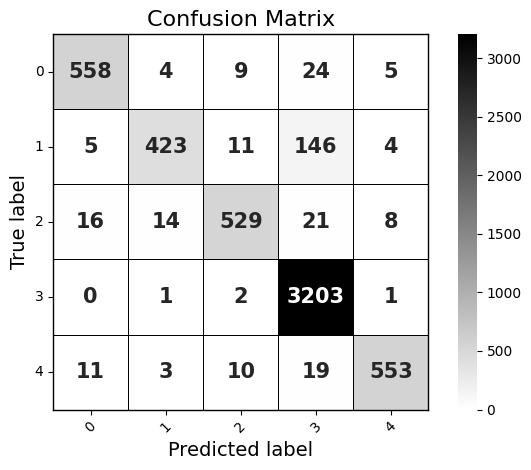
\includegraphics[width=\textwidth]{Images/LR Confusion Matrix.png}
        \caption*{Confusion Matrix (Logistic Regression)}
        \label{LRCM}  % Label for referencing the subfigure
    \end{subfigure}
    \hfill
    \begin{subfigure}[b]{0.49\textwidth}
        \centering
        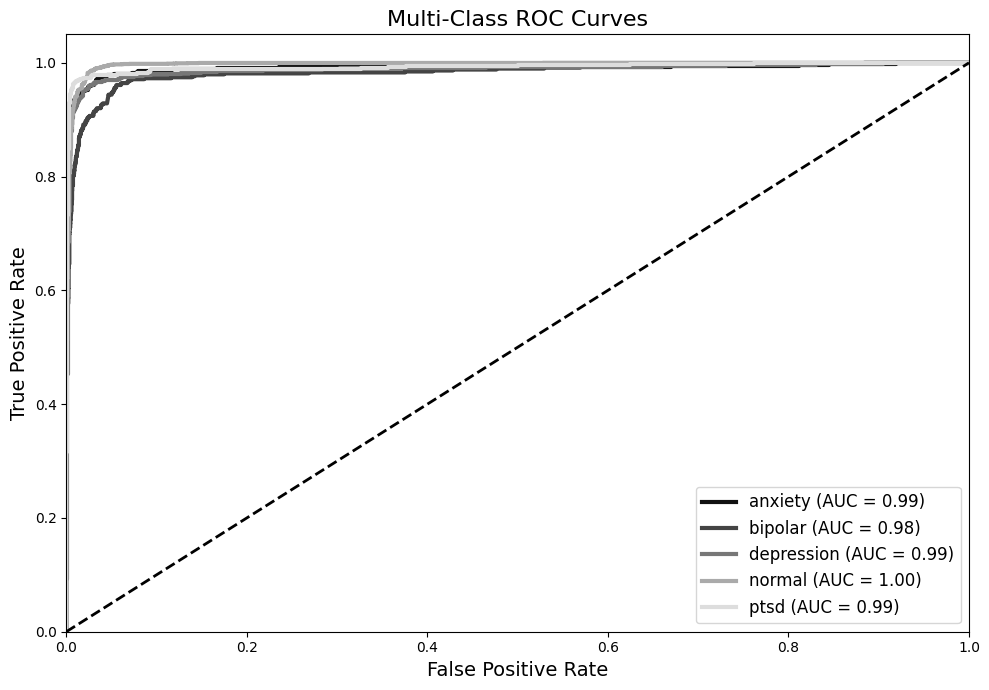
\includegraphics[width=\textwidth]{Images/LR ROC.png}
        \caption*{ROC AUC (Logistic Regression)}
        \label{LRROC}  % Label for referencing the subfigure
    \end{subfigure}
    \label{fig:comparison}
\end{figure}

\begin{figure}[h!]
    \centering
    \begin{subfigure}[b]{0.49\textwidth}
        \centering
        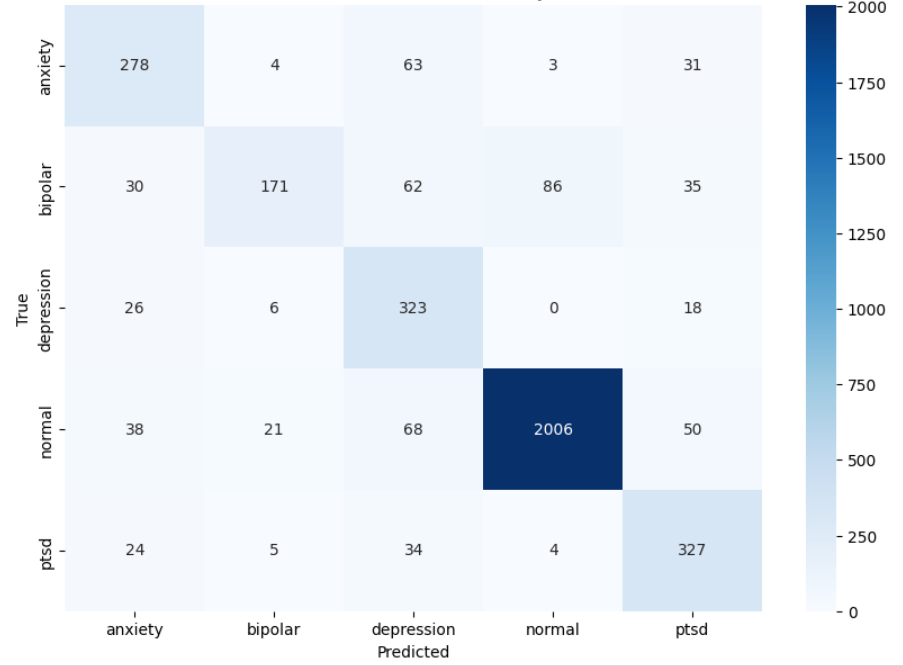
\includegraphics[width=\textwidth]{Images/NB Confusion Matrix.png}
        \caption*{Confusion Matrix (Naive Bayes)}
        \label{NBCM}  % Label for referencing the subfigure
    \end{subfigure}
    \hfill
    \begin{subfigure}[b]{0.49\textwidth}
        \centering
        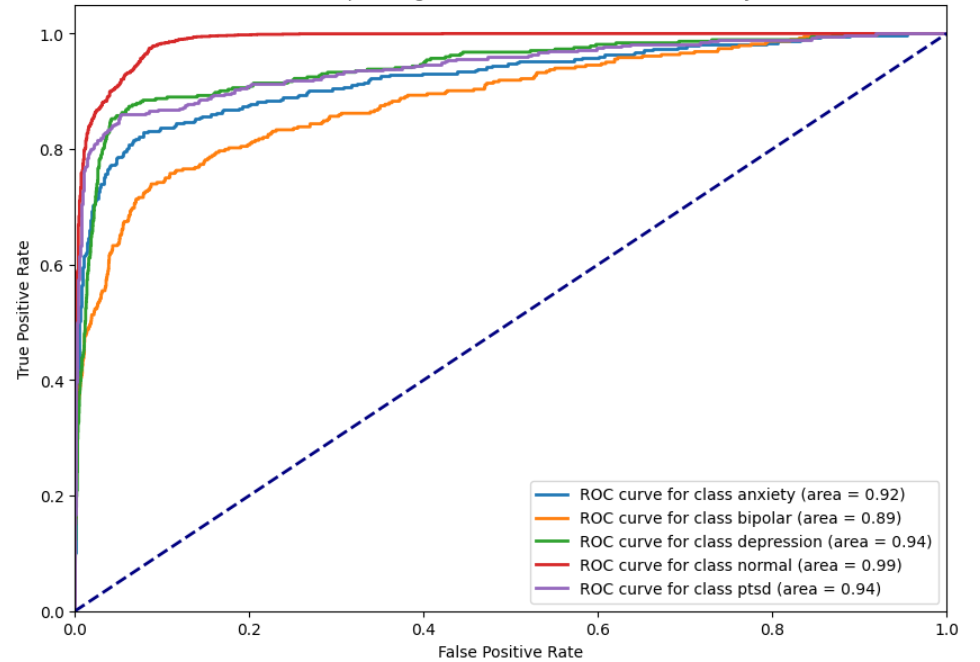
\includegraphics[width=\textwidth]{Images/NB ROC.png}
        \caption*{ROC AUC (Naive Bayes)}
        \label{NBROC}  % Label for referencing the subfigure
    \end{subfigure}
    \label{fig:nb_comparison}
\end{figure}


\begin{figure}[h!]
    \centering
    \begin{subfigure}[b]{0.49\textwidth}
        \centering
        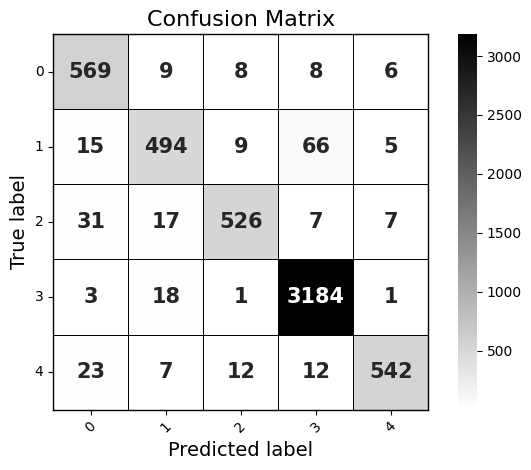
\includegraphics[width=\textwidth]{Images/SVM Confusion Matrix.png}
        \caption*{Confusion Matrix (SVM)}
        \label{SVMCM}  % Label for referencing the subfigure
    \end{subfigure}
    \hfill
    \begin{subfigure}[b]{0.49\textwidth}
        \centering
        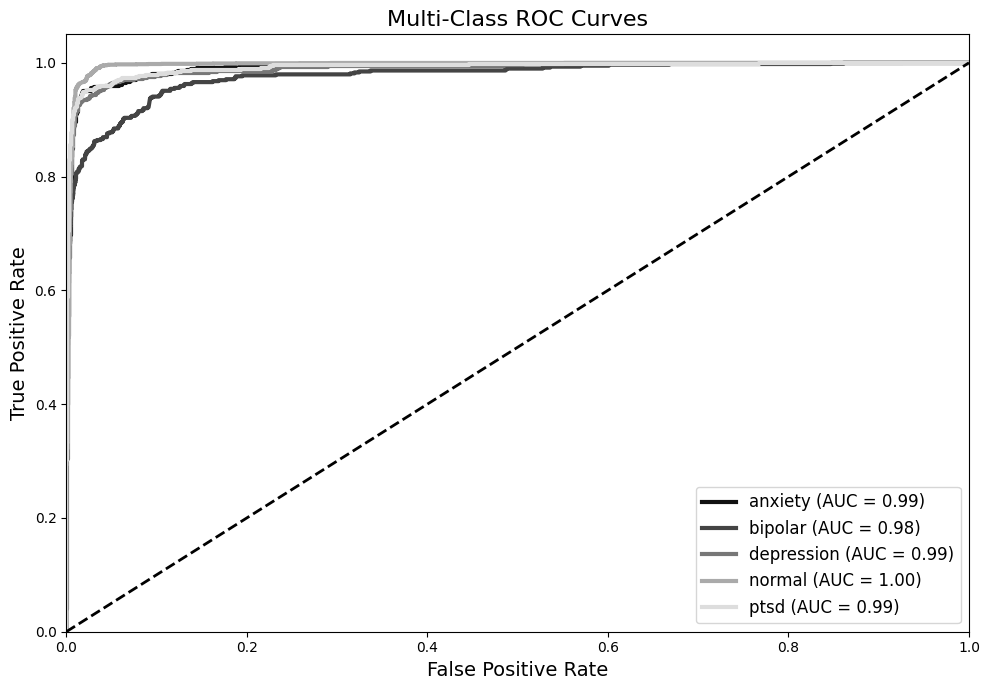
\includegraphics[width=\textwidth]{Images/SVM ROC.png}
        \caption*{ROC AUC (SVM)}
        \label{SVMROC}  % Label for referencing the subfigure
    \end{subfigure}
    \label{fig:svm_comparison}
\end{figure}

\pagebreak

\begin{figure}[h!]
    \centering
    \begin{subfigure}[b]{0.49\textwidth}
        \centering
        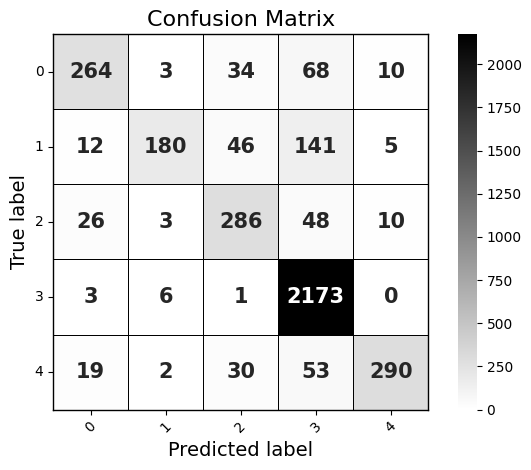
\includegraphics[width=\textwidth]{Images/RF Confusion Matrix.png}
        \caption*{Confusion Matrix (Random Forest)}
        \label{RFCM}  % Label for referencing the subfigure
    \end{subfigure}
    \hfill
    \begin{subfigure}[b]{0.49\textwidth}
        \centering
        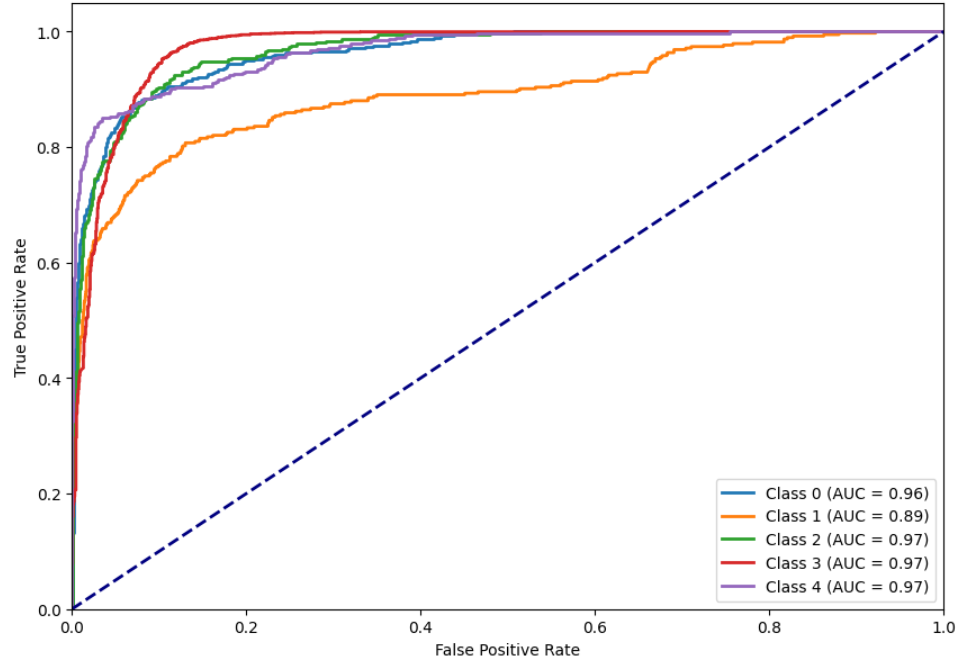
\includegraphics[width=\textwidth]{Images/RF ROC.png}
        \caption*{ROC AUC (Random Forest)}
        \label{RFROC}  % Label for referencing the subfigure
    \end{subfigure}
    \label{fig:rf_comparison}
\end{figure}


\begin{figure}[h!]
    \centering
    \begin{subfigure}[b]{0.49\textwidth}
        \centering
        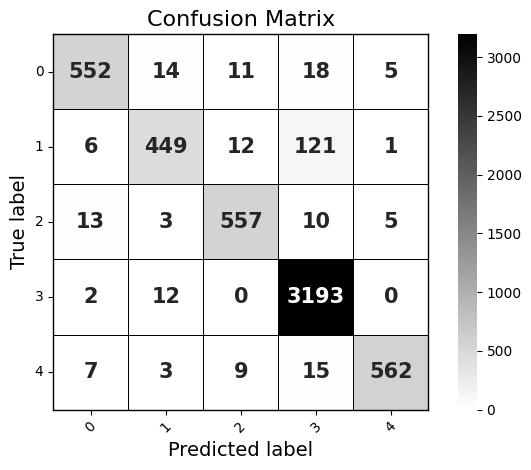
\includegraphics[width=\textwidth]{Images/XG Confusion Matrix.png}
        \caption*{Confusion Matrix (XGBoost)}
        \label{XGCM}  % Label for referencing the subfigure
    \end{subfigure}
    \hfill
    \begin{subfigure}[b]{0.49\textwidth}
        \centering
        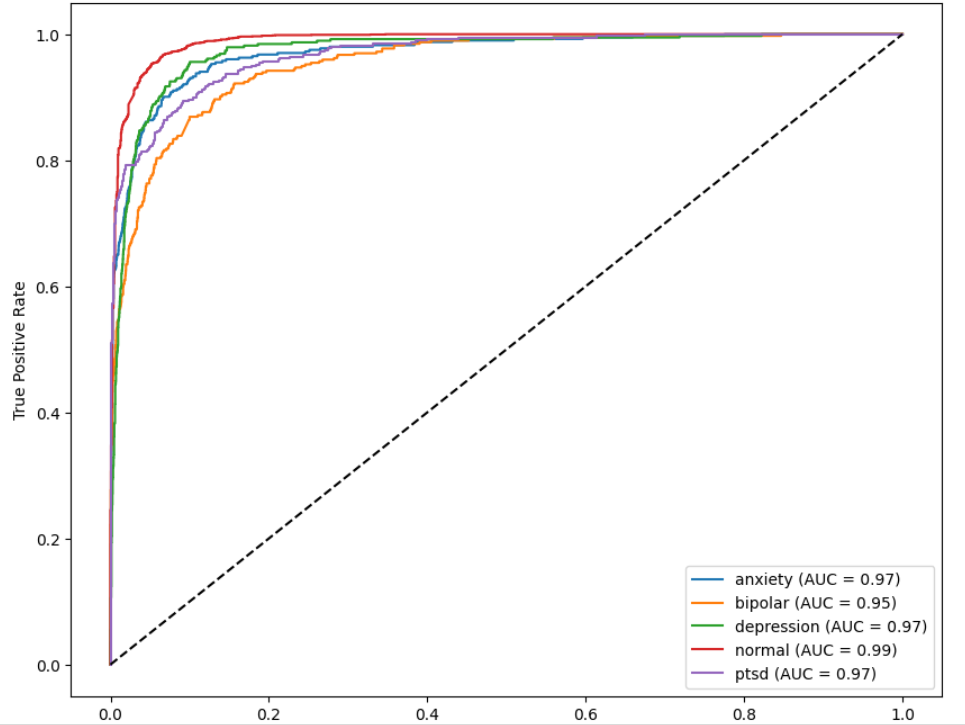
\includegraphics[width=\textwidth]{Images/XG ROC.png}
        \caption*{ROC AUC (XGBoost)}
        \label{XGROC}  % Label for referencing the subfigure
    \end{subfigure}
    \label{fig:xgboost_comparison}
\end{figure}


\begin{figure}[h!]
    \centering
    \begin{subfigure}[b]{0.49\textwidth}
        \centering
        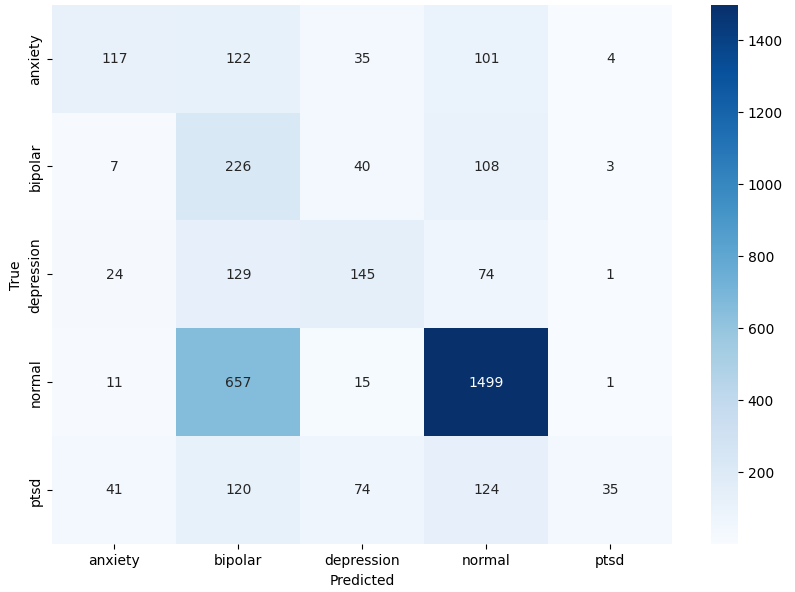
\includegraphics[width=\textwidth]{Images/KNN Confusion Matrix.png}
        \caption*{Confusion Matrix (KNN)}
        \label{KNNCM}  % Label for referencing the subfigure
    \end{subfigure}
    \hfill
    \begin{subfigure}[b]{0.49\textwidth}
        \centering
        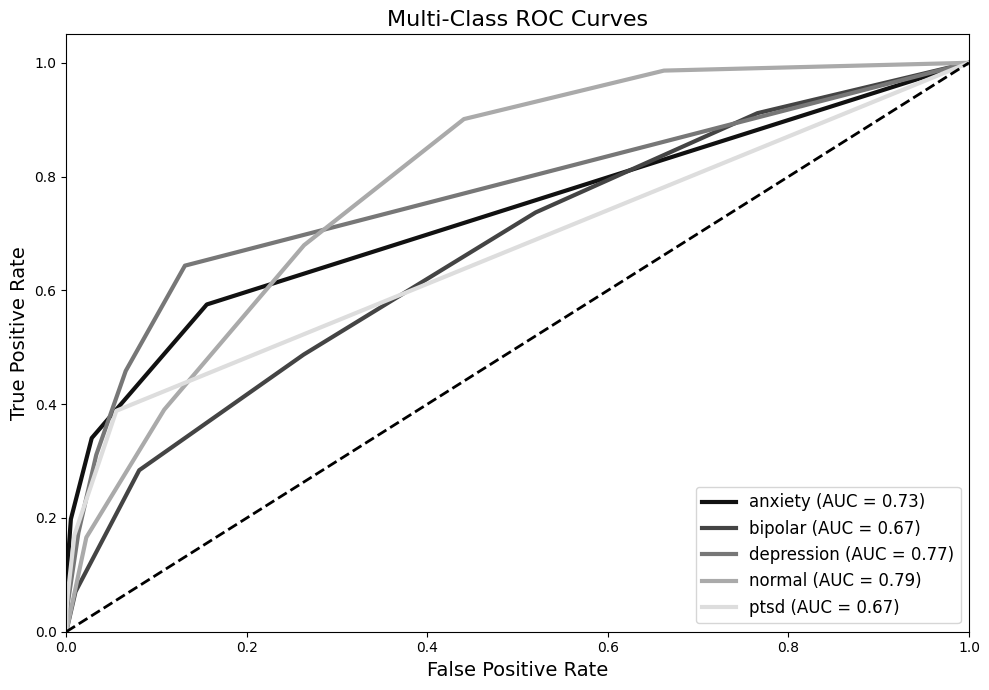
\includegraphics[width=\textwidth]{Images/KNN ROC.png}
        \caption*{ROC AUC (KNN)}
        \label{KNNROC}  % Label for referencing the subfigure
    \end{subfigure}
    \label{fig:knn_comparison}
\end{figure}

\pagebreak

\begin{figure}[h!]
    \centering
    \begin{subfigure}[b]{0.49\textwidth}
        \centering
        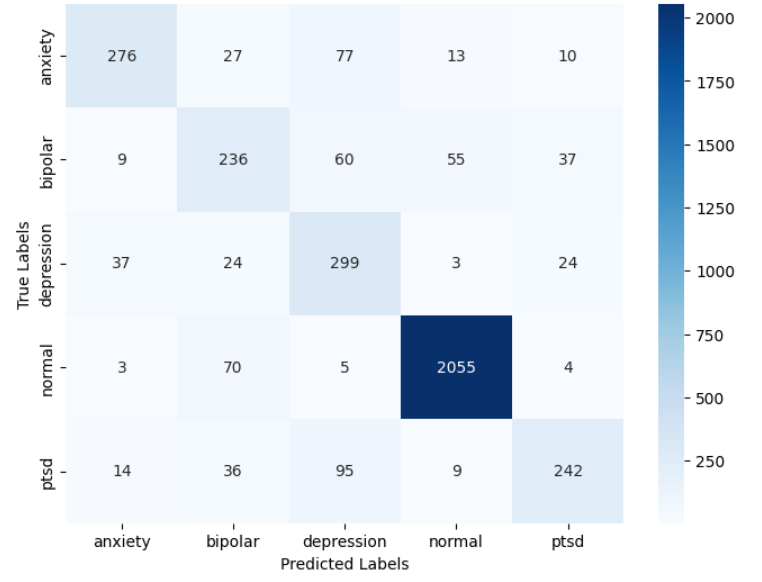
\includegraphics[width=\textwidth]{Images/LSTM Confusion Matrix.png}
        \caption*{Confusion Matrix (LSTM)}
        \label{LSTMCM}  % Label for referencing the subfigure
    \end{subfigure}
    \hfill
    \begin{subfigure}[b]{0.49\textwidth}
        \centering
        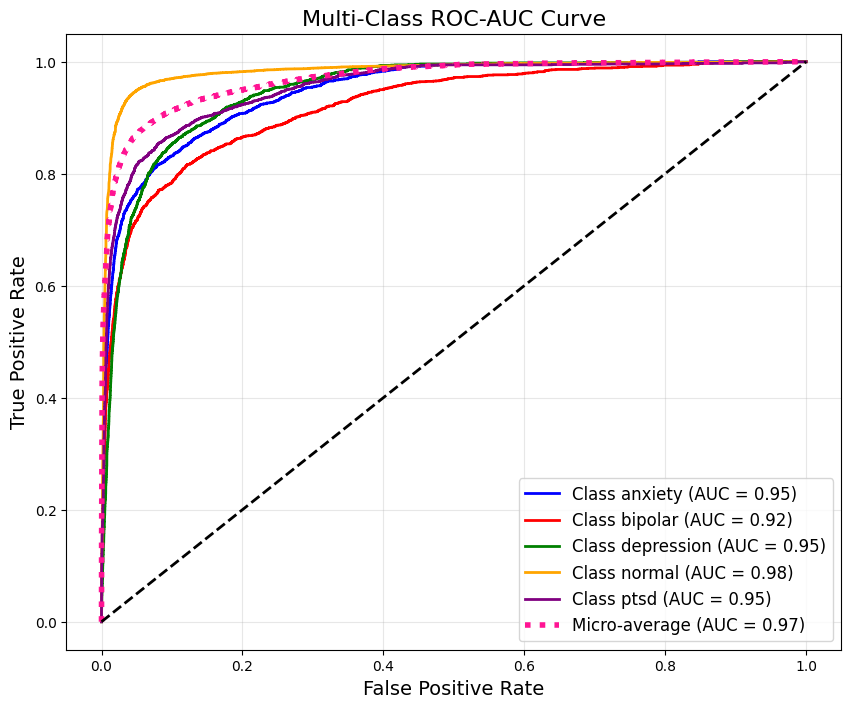
\includegraphics[width=\textwidth]{Images/LSTM ROC.png}
        \caption*{ROC AUC (LSTM)}
        \label{LSTMROC}  % Label for referencing the subfigure
    \end{subfigure}
    \label{fig:lstm_comparison}
\end{figure}


\begin{figure}[h!]
    \centering
    \begin{subfigure}[b]{0.49\textwidth}
        \centering
        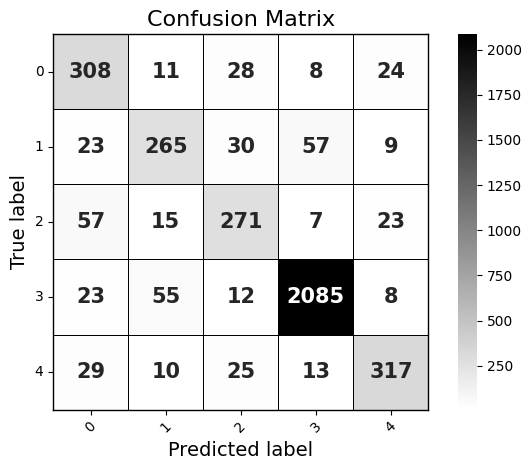
\includegraphics[width=\textwidth]{Images/T CM.png}
        \caption*{Confusion Matrix (Transformer based Model)}
        \label{dfdl145}  % Label for referencing the subfigure
    \end{subfigure}
    \hfill
    \begin{subfigure}[b]{0.49\textwidth}
        \centering
        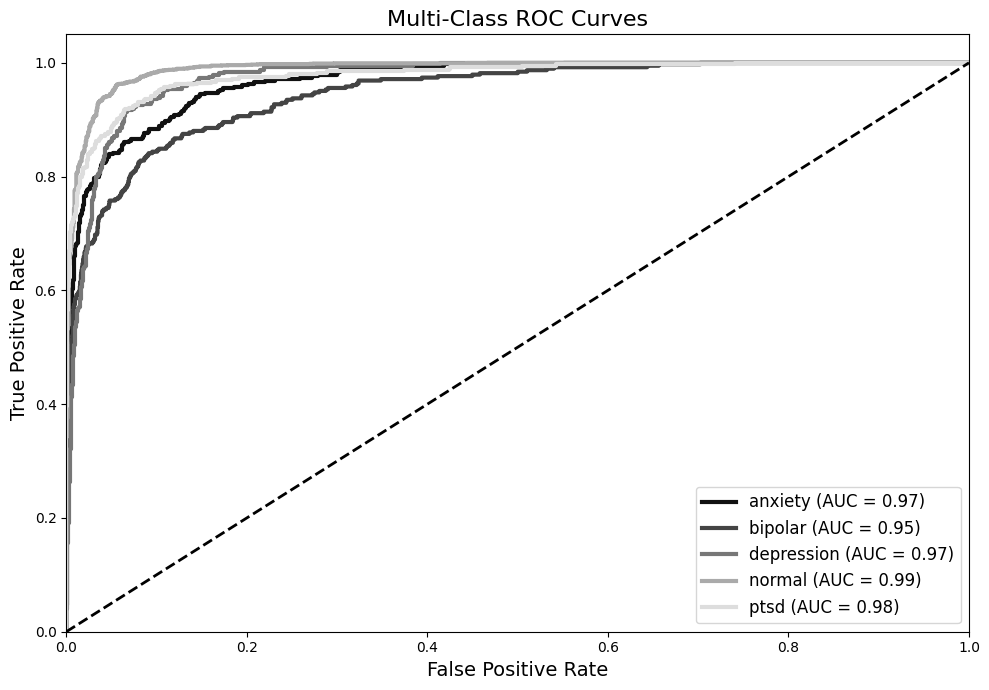
\includegraphics[width=\textwidth]{Images/T ROC.png}
        \caption*{ROC AUC (Transformer based Model)}
        \label{dfdl146}  % Updated label for referencing the subfigure
    \end{subfigure}
    \label{fig:transformer_comparison}
\end{figure}


\begin{figure}[h!]
    \centering
    \begin{subfigure}[b]{0.49\textwidth}
        \centering
        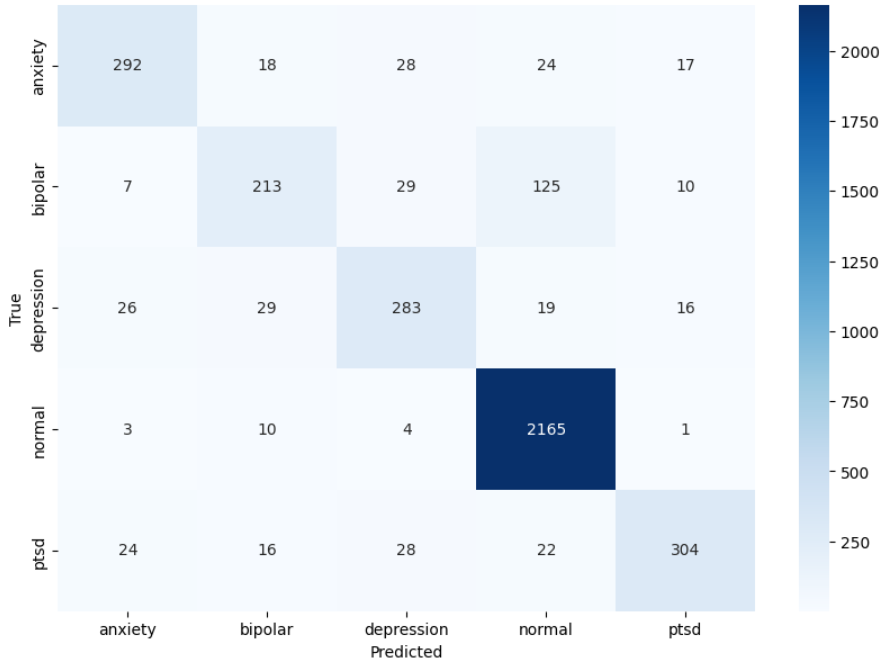
\includegraphics[width=\textwidth]{Images/HP LR CM.png}
        \label{LSTMROC2}  % Label for referencing the subfigure
    \end{subfigure}
    \hfill
    \begin{subfigure}[b]{0.49\textwidth}
        \centering
        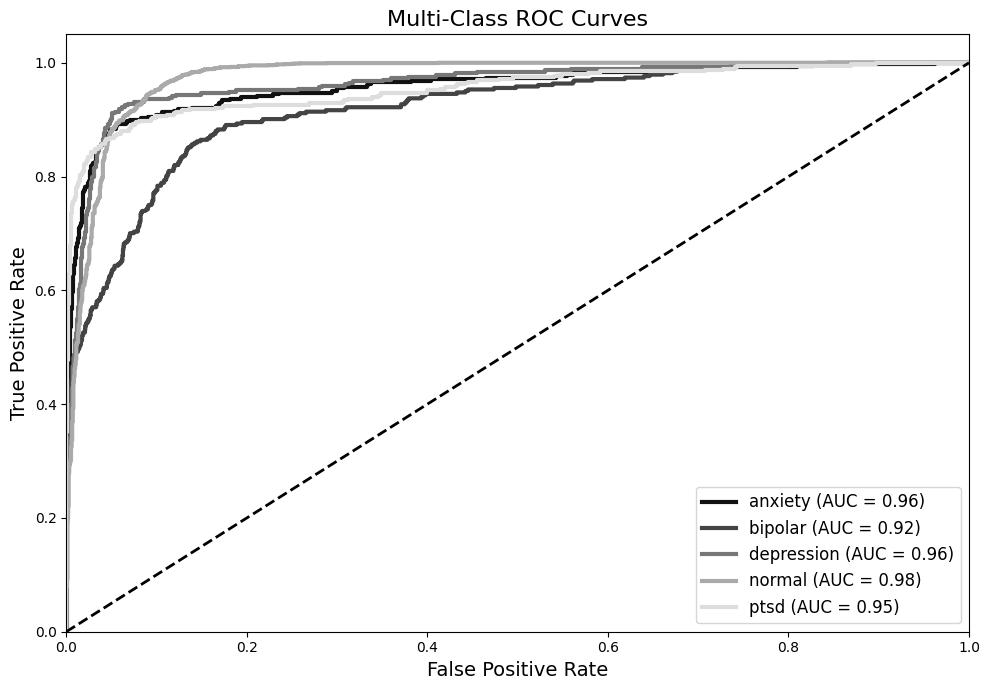
\includegraphics[width=\textwidth]{Images/HP LR ROC.png}
        \label{LSTMROC3}  % Label for referencing the subfigure
    \end{subfigure}
    \vspace{-2em}
    \caption*{Confusion Matrix and ROC AUC for Logistic Regression with Hyperparameter Tuning}
    \label{fig:hp_lr_comparison}
\end{figure}

\pagebreak

\begin{figure}[h!]
    \centering
    \begin{subfigure}[b]{0.49\textwidth}
        \centering
        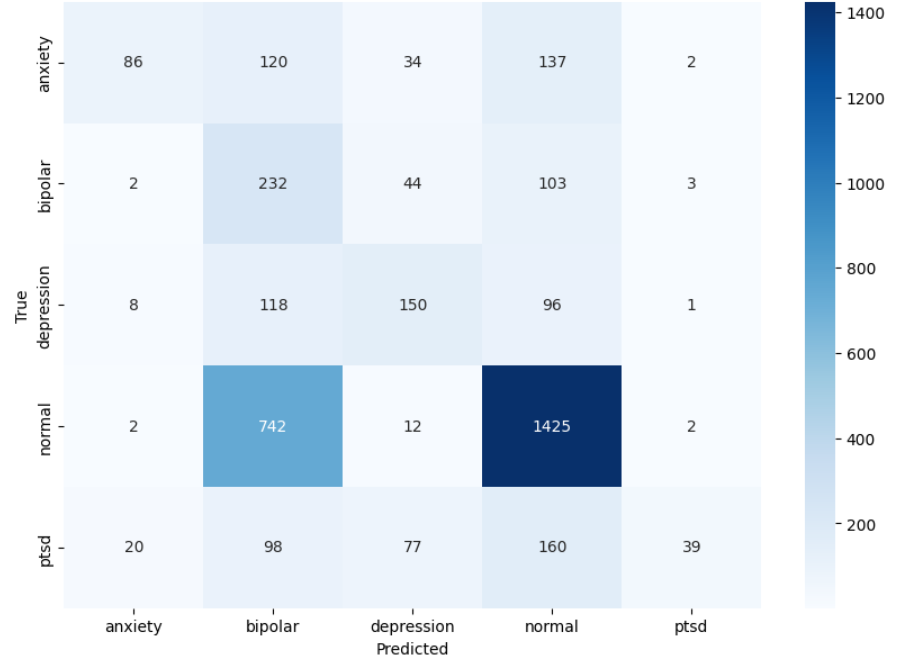
\includegraphics[width=\textwidth]{Images/HP KNN CM.png}
        \label{LSTMROC4}  % Label for referencing the subfigure
    \end{subfigure}
    \hfill
    \begin{subfigure}[b]{0.49\textwidth}
        \centering
        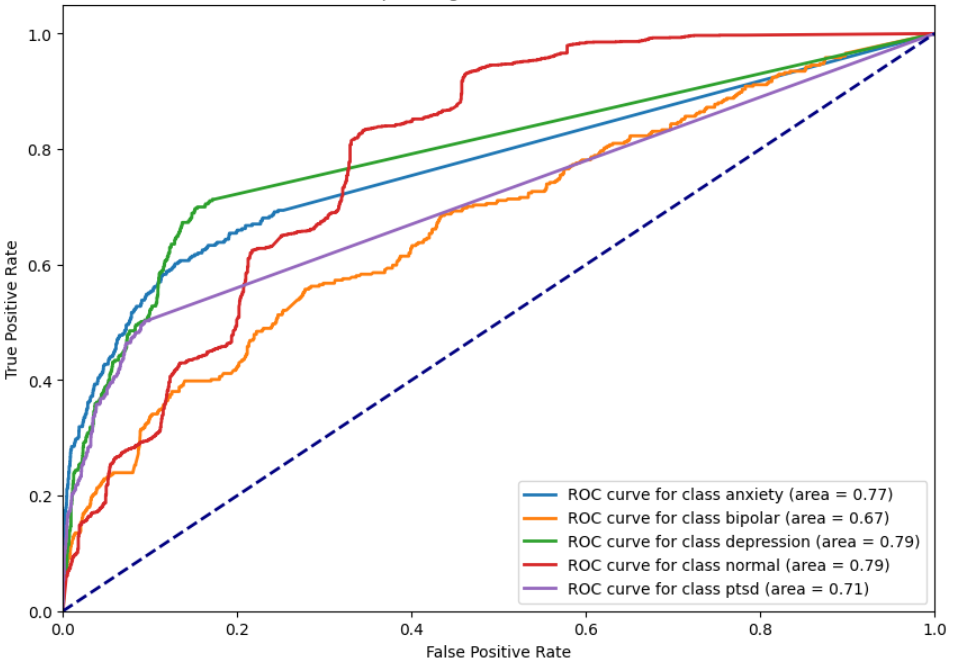
\includegraphics[width=\textwidth]{Images/HP KNN ROC.png}
        \label{LSTMROC5}  % Label for referencing the subfigure
    \end{subfigure}
    \vspace{-1.5em}
    \caption*{Confusion Matrix and ROC AUC for KNN with Hyperparameter Tuning}
    \label{fig:hp_knn_comparison}
\end{figure}



\begin{figure}[h!]
    \centering
    \begin{subfigure}[b]{0.49\textwidth}
        \centering
        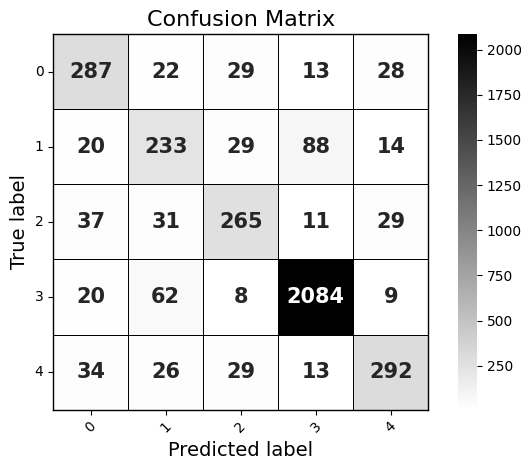
\includegraphics[width=\textwidth]{Images/HP SVM CM.png}
        \label{LSTMROC6}  % Label for referencing the subfigure
    \end{subfigure}
    \hfill
    \begin{subfigure}[b]{0.49\textwidth}
        \centering
        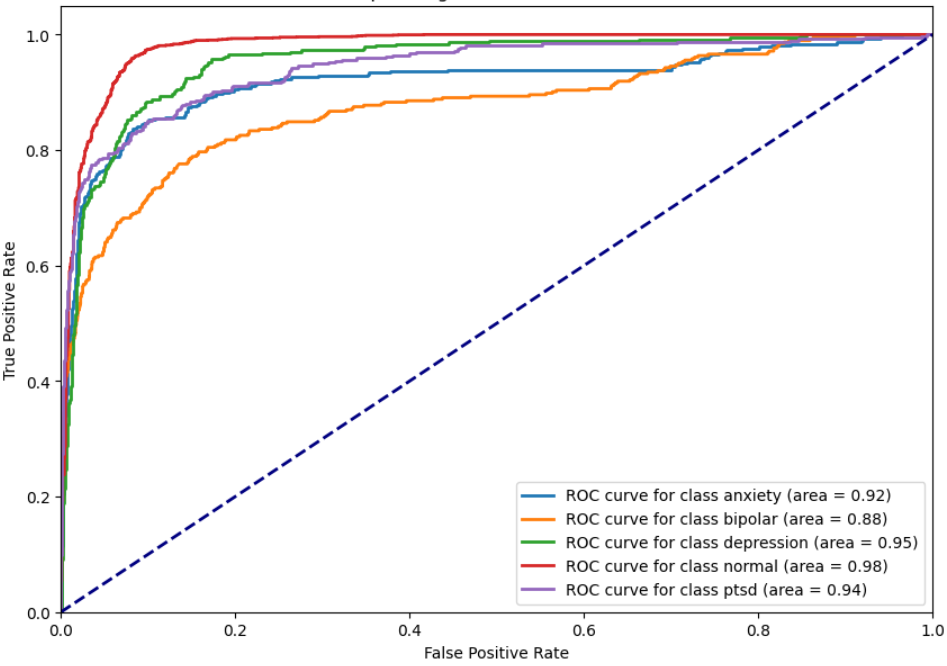
\includegraphics[width=\textwidth]{Images/HP SVM ROC.png}
        \label{LSTMROC}  % Label for referencing the subfigure
    \end{subfigure}
    \vspace{-1.5em}
    \caption*{Confusion Matrix and ROC AUC for SVM with Hyperparameter Tuning}
    \label{fig:hp_svm_comparison}
\end{figure}


\begin{figure}[h!]
    \centering
    \begin{subfigure}[b]{0.49\textwidth}
        \centering
        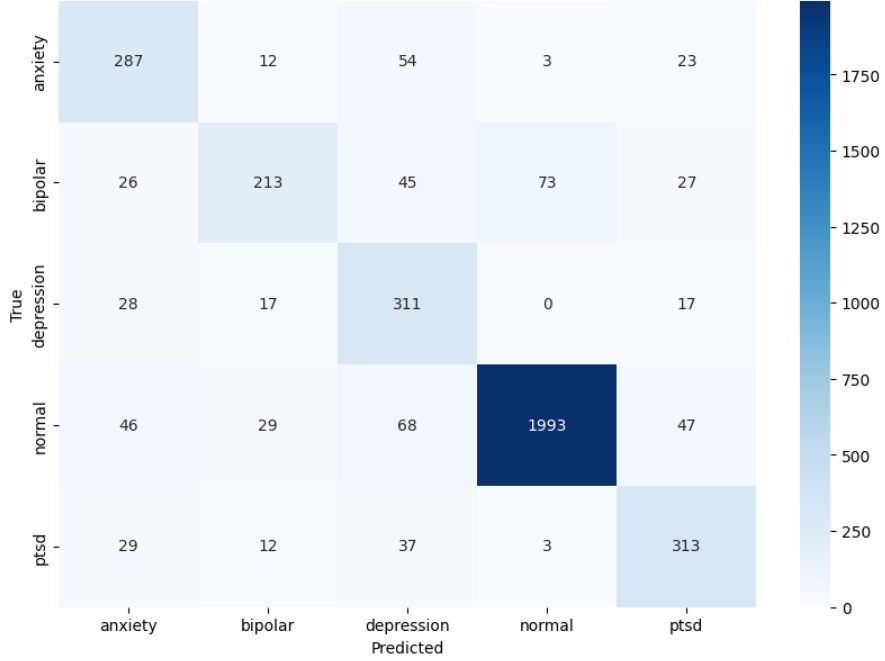
\includegraphics[width=\textwidth]{Images/HP NB CM.png}
        \label{LSTMROC7}  % Label for referencing the subfigure
    \end{subfigure}
    \hfill
    \begin{subfigure}[b]{0.49\textwidth}
        \centering
        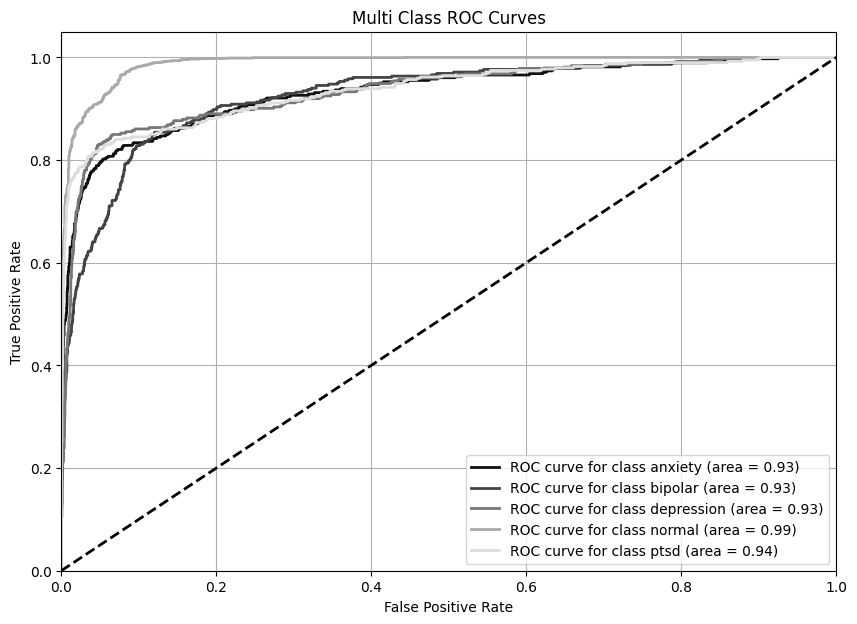
\includegraphics[width=\textwidth]{Images/HP NB ROC.png}
        \label{LSTMROC8}  % Label for referencing the subfigure
    \end{subfigure}
    \vspace{-1.5em}
    \caption*{Confusion Matrix and ROC AUC for Naive Bayes with Hyperparameter Tuning}
    \label{fig:hp_nb_comparison}
\end{figure}


\pagebreak

\begin{table}[H]
    \centering
    \renewcommand{\arraystretch}{1.2}
    \small
    \begin{tabularx}{\textwidth}{|l|c|X|}
    \hline
    \textbf{Model} & \textbf{Accuracy (\%)} & \textbf{Key Observations} \\
    \hline
    Logistic Regression & 87.66 & High precision, recall, and F1 for the \textit{Normal} class; struggles with \textit{Bipolar} and \textit{Anxiety}. ROC AUC: Normal (0.99), Anxiety (0.95), Depression (0.96). \\
    \hline
    Naive Bayes & 83.63 & Excellent for \textit{Normal} (Precision 0.96, Recall 0.92, F1 0.94) but poor for \textit{Bipolar} (Recall 0.45, F1 0.58). \newline ROC AUC: Normal (0.99), Depression/PTSD (0.94), Bipolar (0.89). \\
    \hline
    SVM & 85.13 & Best for \textit{Normal} (Precision 0.94, Recall 0.95, F1 0.95); \textit{Bipolar} underperforms (Precision 0.62, Recall 0.61); \textit{Anxiety} is balanced (Recall 0.76, Precision 0.72). \newline ROC AUC: Normal (0.98), others ~0.96, Bipolar (0.90). \\
    \hline
    Random Forest & 86.00 & \textit{Normal} class achieves perfect recall (1.00) with high precision (0.88, F1 0.93); \textit{Bipolar} is weak (Recall 0.47, F1 0.62). \newline ROC AUC: For most classes it is greater than equal to 0.96; Bipolar (0.89). \\
    \hline
    XGBoost & 87.39 & Strong performance for \textit{Normal}; \textit{Anxiety} shows good metrics (Precision 0.81, Recall 0.74) while \textit{Bipolar} has lower recall (0.62). \newline ROC AUC: 0.97 for Anxiety, Depression, PTSD; 0.99 for Normal. \\
    \hline
    KNN & 54.46 & Overall low performance; \textit{Normal} is moderate (Precision 0.79, Recall 0.69) but \textit{PTSD} has very low recall (0.09). \newline ROC AUC: Normal (0.80), indicating weak discrimination. \\
    \hline
    LSTM & 84.91 & High performance for \textit{Normal}; \textit{Anxiety} acceptable (Precision 0.74, Recall 0.72); \textit{Bipolar} (Precision 0.66, Recall 0.70) and \textit{PTSD} (Precision 0.72, Recall 0.78) are moderate. \newline Effective ROC AUC for Normal. \\
    \hline
    Transformer & 88.50 & Best overall with balanced high precision and recall across all classes. Captures contextual cues effectively and handles class imbalance well. \newline ROC AUC scores range between 0.94 and 0.99. \\
    \hline
    \end{tabularx}
    \caption*{\textbf{Summary Comparison of  Classification Models without Hyperparameter Tuning}}
    \label{tab:model_comparison}
\end{table}



\pagebreak

\begin{table}[H]
    \centering
    \renewcommand{\arraystretch}{1.3}
    \small
    \begin{tabularx}{\textwidth}{|l|X|X|X|}
        \hline
        \textbf{Model} & \textbf{Best Hyperparameters} & \textbf{Accuracy \& Metrics} & \textbf{Key Observations} \\
        \hline
        Logistic Regression & \texttt{solver=liblinear, penalty=l2, C=1} & Accuracy: 87.72\%; Normal: 92\% accuracy; ROC AUC: Normal 0.99, Depression 0.96 & High precision, recall, and F1 for Normal; Bipolar shows lower F1 (64\%); overall robust performance, especially for Normal and Anxiety. \\
        \hline
        k-NN & \texttt{weights=distance, n\_neighbors=10, metric=euclidean} & Accuracy: 52.03\%; Normal F1: 0.69; ROC AUC: Bipolar 0.67, PTSD 0.71, Normal/Depression 0.79 & Struggles with minority classes: Anxiety (recall 0.23) and PTSD (recall 0.10); not suitable for this dataset. \\
        \hline
        SVM & \texttt{kernel=linear, gamma=scale, C=1} & Accuracy: 85.13\%; F1-scores: Normal 0.95, Depression 0.72, Anxiety 0.74, Bipolar 0.61; ROC AUC: Normal 0.98, Others \textgreater 0.90, Bipolar 0.90 & Solid overall performance; excellent for Normal and Anxiety, but slightly lower performance for Bipolar. \\
        \hline
        Naive Bayes & \texttt{alpha=0.2914} & Accuracy: 83.95\%; F1-scores: Normal 0.94, PTSD 0.76, Anxiety 0.72; ROC AUC: Normal 0.99, Others \textgreater 0.90 & Performs very well for Normal and PTSD; lower scores for Bipolar and Depression. \\
        \hline
    \end{tabularx}
    \caption*{\textbf{Summary Comparison of Models after Hyperparameter Tuning}}
    \label{tab:hp_tuning_summary}
\end{table}

\vspace{1em}

\noindent
K-Nearest Neighbors (KNN) performs poorly on this mental health dataset compared to other algorithms, even after hyperparameter tuning. KNN relies on distance-based metrics, which struggle with the sparse, high-dimensional nature of text data, making it difficult to capture meaningful relationships between Reddit posts and mental health labels. Despite optimizing parameters like \verb|weights='distance'|, \verb|n_neighbors=10|, and \verb|metric='euclidean'|, KNN's performance remains suboptimal, with lower accuracy, precision, recall, and F1-score than Logistic Regression, Naive Bayes, or SVM. Its inability to handle non-linear, context-dependent patterns in text, especially for nuanced categories like anxiety, PTSD, or bipolar disorder, highlights its limitations in text classification tasks. KNN's reliance on proximity without considering textual context likely explains its poor performance.

\pagebreak

\begin{figure}[h!]  
    \centering
    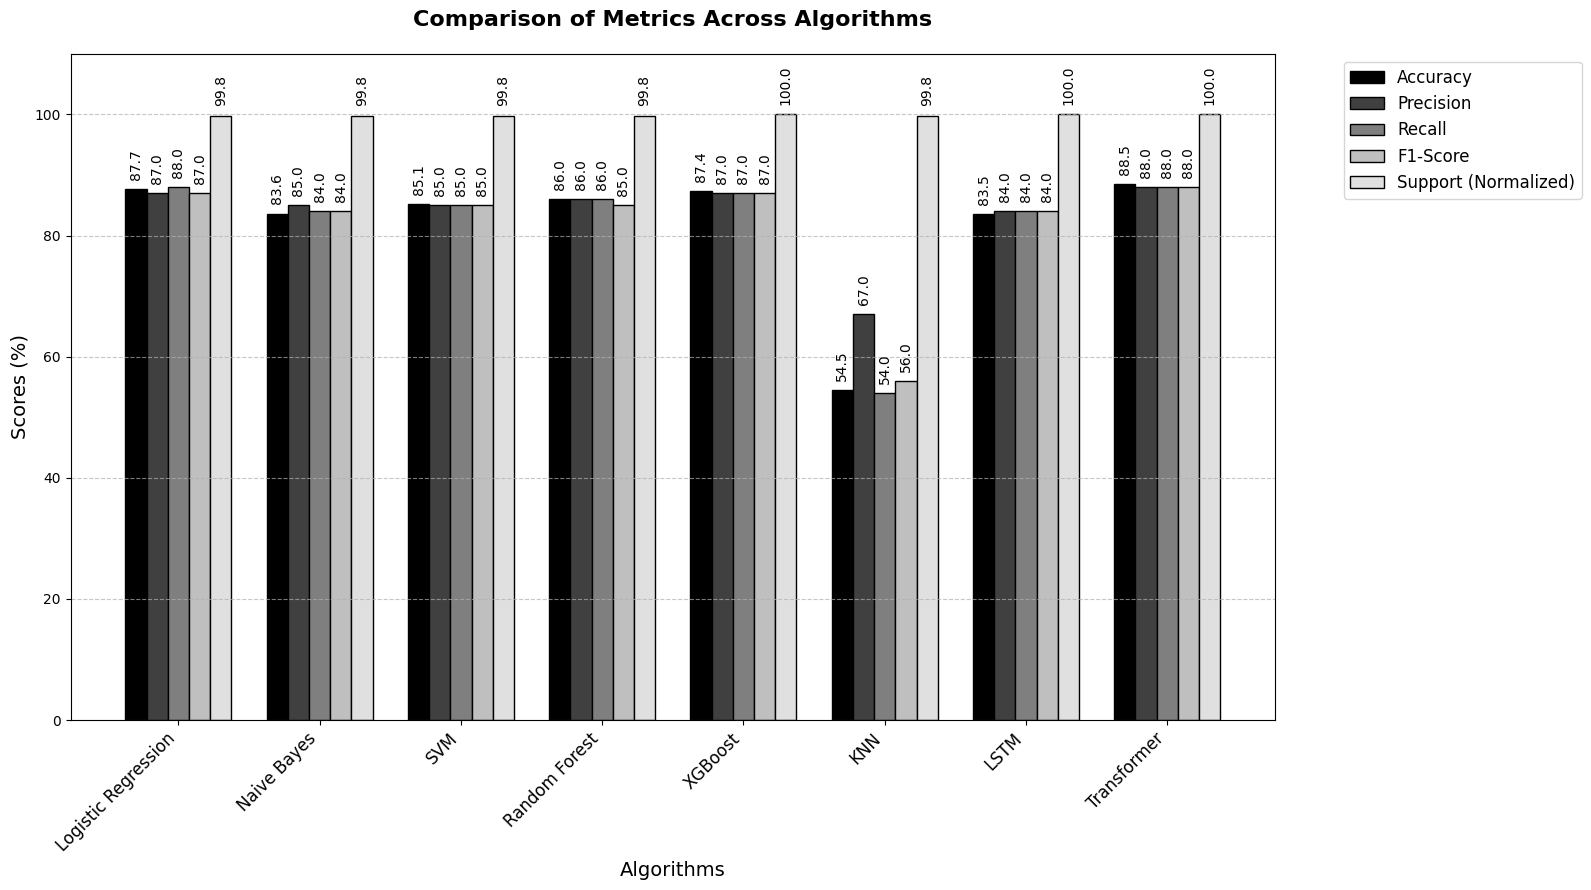
\includegraphics[width=1.0\textwidth]{Images/ML GRAPH 1.png}  
    \caption*{Result Comparison of the Algorithms}
    \label{dfdl145}  % Label for referencing the figure
\end{figure}

\begin{figure}[h!]  
    \centering
    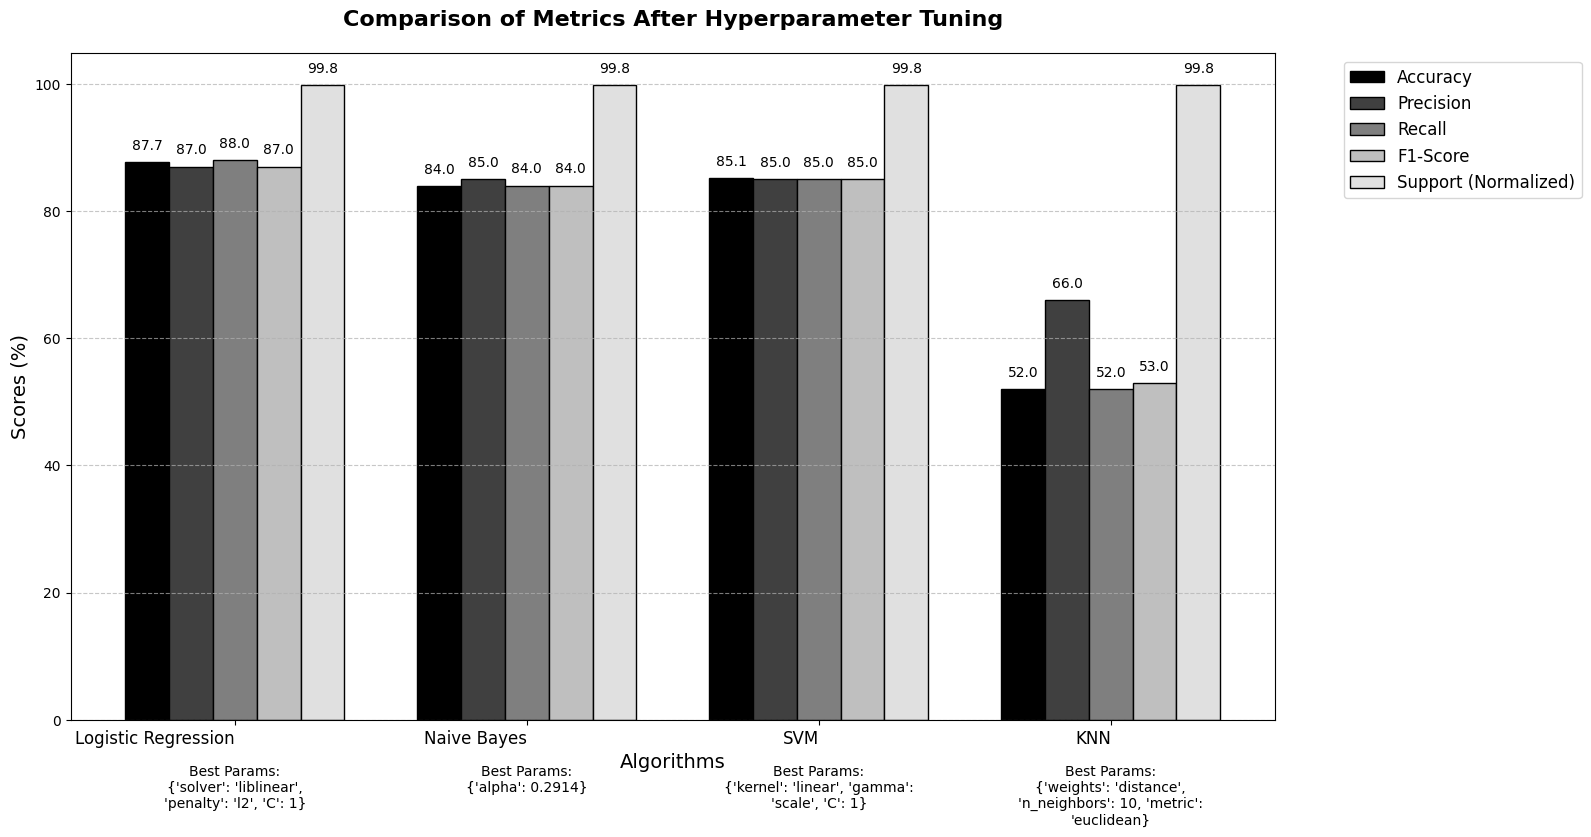
\includegraphics[width=1.0\textwidth]{Images/ML GRAPH 2 HT.png}  
    \caption*{Result Comparison after Hyperparameter Tuning}
    \label{dfdl123}  % Label for referencing the figure
\end{figure}

\pagebreak

% ------------------ Different Vectorization ---------
\subsection{Comparison of different tokenizations}
\begin{center}
    \textbf{Model Performance Comparison} \\[0.5em]
    \begin{tabular}{|c|c|c|c|c|c|}
        \hline
        \textbf{Model} & \textbf{BoW} & \textbf{TFIDF} & \textbf{LIWC} & \textbf{Word2Vec} & \textbf{N-Gram} \\ \hline
        \textbf{Logistic Regression} & 87.66 & 86.02 & 66.36 & 79.40 & 87.13 \\ \hline
        \textbf{KNN} & 54.56 & 75.06 & 70.70 & 75.52 & 43.06 \\ \hline
        \textbf{SVC} & 85.13 & 88.26 & 68.14 & 77.89 & 84.33 \\ \hline
        \textbf{Naive Bayes} & 83.63 & 79.42 & 59.63 & 60.44 & 81.71 \\ \hline
        \textbf{Random Forest} & 85.32 & 85.73 & 76.73 & 79.88 & 79.02 \\ \hline
        \textbf{XGB} & 87.42 & 87.39 & 78.56 & 81.01 & 87.96 \\ \hline
    \end{tabular}
\end{center}

\noindent
In ensemble learning, combining models like Logistic Regression (LR), Naive Bayes (NB), K-Nearest Neighbors (KNN), Support Vector Machine (SVM), XGBoost (XGB), Random Forest (RF), and Long Short-Term Memory (LSTM) poses challenges in computational efficiency, model size, and accuracy. Each model has unique strengths and limitations, making their integration complex. LR, NB, and SVM perform well with simpler vectorization methods like Bag of Words (BoW), which efficiently represents text data as sparse vectors. BoW’s simplicity ensures these models remain computationally lightweight while maintaining good classification accuracy. In contrast, XGBoost benefits from more complex feature extraction methods like TFIDF (Term Frequency-Inverse Document Frequency), which captures nuanced relationships by weighting words based on their importance across documents. However, combining TFIDF-based models like XGBoost with BoW-based models can degrade ensemble performance, as the feature representations may not align well. KNN is excluded due to its computational intensity, as it requires storing the entire training dataset and performs poorly with large, high-dimensional datasets. Similarly, Random Forest is omitted because its multiple decision trees increase model size and inference time, outweighing its individual performance benefits. XGBoost, while highly accurate with N-Gram features, is computationally expensive and impractical for real-time systems or large-scale deployment. The choice of feature extraction methods—BoW for LR, NB, and SVM, and TFIDF for XGBoost—balances simplicity and complexity. BoW ensures efficient, interpretable representations for simpler models, while TFIDF provides richer, context-aware features for XGBoost. This combination leverages the strengths of both methods, ensuring each model operates effectively without excessive computational strain. Ultimately, this approach strikes a balance between accuracy and efficiency, enabling the ensemble to perform well while remaining scalable and practical for real-world applications.
\pagebreak

\subsection{Results from Ensemble Model Training and Testing}

\begin{center}
    \textbf{Ensemble Model 1} \\[0.2em]
    \begin{tabular}{|c|c|c|c|c|}
        \hline
        & \textbf{Precision} & \textbf{Recall} & \textbf{F1-Score} & \textbf{Support} \\ \hline
        \textbf{Anxiety}    & 0.97 & 0.94 & 0.95 & 400  \\ \hline
        \textbf{Bipolar}    & 0.92 & 0.85 & 0.88 & 388  \\ \hline
        \textbf{Depression} & 0.95 & 0.94 & 0.94 & 392  \\ \hline
        \textbf{Normal}     & 0.97 & 0.99 & 0.98 & 2136 \\ \hline
        \textbf{PTSD}       & 0.97 & 0.96 & 0.96 & 397  \\ \hline
        \textbf{Accuracy}   & \multicolumn{4}{|c|}{\textbf{96.08\%}} \\ \hline
        \textbf{Macro avg}  & 0.96 & 0.93 & 0.95 & 3713 \\ \hline
        \textbf{Weighted avg} & 0.96 & 0.96 & 0.96 & 3713 \\ \hline
    \end{tabular}
\end{center}


\begin{center}
    \textbf{Ensemble Model 2} \\[0.2em]
    \begin{tabular}{|c|c|c|c|c|}
        \hline
        & \textbf{Precision} & \textbf{Recall} & \textbf{F1-Score} & \textbf{Support} \\ \hline
        \textbf{Anxiety}    & 0.97 & 0.97 & 0.97 & 400  \\ \hline
        \textbf{Bipolar}    & 0.95 & 0.92 & 0.93 & 388  \\ \hline
        \textbf{Depression} & 0.98 & 0.96 & 0.97 & 392  \\ \hline
        \textbf{Normal}     & 0.99 & 0.99 & 0.99 & 2136 \\ \hline
        \textbf{PTSD}       & 0.97 & 0.98 & 0.98 & 397  \\ \hline
        \textbf{Accuracy}   & \multicolumn{4}{|c|}{\textbf{97.93\%}} \\ \hline
        \textbf{Macro avg}  & 0.97 & 0.97 & 0.97 & 3713 \\ \hline
        \textbf{Weighted avg} & 0.98 & 0.98 & 0.98 & 3713 \\ \hline
    \end{tabular}
\end{center}


\begin{center}
    \textbf{Ensemble Model 3} \\[0.2em]
    \begin{tabular}{|c|c|c|c|c|}
        \hline
        & \textbf{Precision} & \textbf{Recall} & \textbf{F1-Score} & \textbf{Support} \\ \hline
        \textbf{Anxiety}    & 0.98 & 0.97 & 0.98 & 400  \\ \hline
        \textbf{Bipolar}    & 0.96 & 0.90 & 0.93 & 388  \\ \hline
        \textbf{Depression} & 0.97 & 0.96 & 0.96 & 392  \\ \hline
        \textbf{Normal}     & 0.98 & 1.00 & 0.99 & 2136 \\ \hline
        \textbf{PTSD}       & 0.97 & 0.97 & 0.97 & 397  \\ \hline
        \textbf{Accuracy}   & \multicolumn{4}{|c|}{\textbf{97.76\%}} \\ \hline
        \textbf{Macro avg}  & 0.97 & 0.96 & 0.97 & 3713 \\ \hline
        \textbf{Weighted avg} & 0.98 & 0.98 & 0.98 & 3713 \\ \hline
    \end{tabular}
\end{center}


\begin{center}
    \textbf{Ensemble Model 4} \\[0.2em]
    \begin{tabular}{|c|c|c|c|c|}
        \hline
        \textbf{Class} & \textbf{Precision} & \textbf{Recall} & \textbf{F1-Score} & \textbf{Support} \\ \hline
        Anxiety & 0.97 & 0.97 & 0.97 & 400 \\ \hline
        Bipolar & 0.95 & 0.90 & 0.92 & 388 \\ \hline
        Depression & 0.97 & 0.95 & 0.96 & 392 \\ \hline
        Normal & 0.99 & 0.99 & 0.99 & 2136 \\ \hline
        PTSD & 0.97 & 0.98 & 0.97 & 397 \\ \hline
        \textbf{Accuracy} & \multicolumn{4}{c|}{\textbf{97.63\%}} \\ \hline
        \textbf{Macro Avg} & 0.97 & 0.96 & 0.96 & 3713 \\ \hline
        \textbf{Weighted Avg} & 0.98 & 0.98 & 0.98 & 3713 \\ \hline
    \end{tabular}
\end{center}



\pagebreak


\begin{center}
    \textbf{Ensemble Model 5} \\[0.2em]
    \begin{tabular}{|c|c|c|c|c|}
        \hline
        & \textbf{Precision} & \textbf{Recall} & \textbf{F1-Score} & \textbf{Support} \\ \hline
        \textbf{Anxiety}    & 0.96 & 0.95 & 0.96 & 400 \\ \hline
        \textbf{Bipolar}    & 0.94 & 0.89 & 0.92 & 388 \\ \hline
        \textbf{Depression} & 0.96 & 0.95 & 0.95 & 392 \\ \hline
        \textbf{Normal}     & 0.98 & 0.99 & 0.99 & 2136 \\ \hline
        \textbf{PTSD}       & 0.97 & 0.97 & 0.97 & 397 \\ \hline
        \textbf{Accuracy}   & \multicolumn{4}{c|}{\textbf{97.17\%}} \\ \hline
        \textbf{Macro avg}  & 0.96 & 0.95 & 0.96 & 3713 \\ \hline
        \textbf{Weighted avg} & 0.97 & 0.97 & 0.97 & 3713 \\ \hline
    \end{tabular}
\end{center}


\begin{center}
    \textbf{Ensemble Model 6} \\[0.2em]
    \begin{tabular}{|c|c|c|c|c|}
        \hline
        & \textbf{Precision} & \textbf{Recall} & \textbf{F1-Score} & \textbf{Support} \\ \hline
        \textbf{Anxiety}    & 0.95 & 0.92 & 0.94 & 400 \\ \hline
        \textbf{Bipolar}    & 0.96 & 0.74 & 0.84 & 388 \\ \hline
        \textbf{Depression} & 0.92 & 0.94 & 0.93 & 392 \\ \hline
        \textbf{Normal}     & 0.95 & 1.00 & 0.97 & 2136 \\ \hline
        \textbf{PTSD}       & 0.98 & 0.93 & 0.96 & 397 \\ \hline
        \textbf{Accuracy}   & \multicolumn{4}{c|}{\textbf{95.15\%}} \\ \hline
        \textbf{Macro avg}  & 0.95 & 0.91 & 0.93 & 3713 \\ \hline
        \textbf{Weighted avg} & 0.95 & 0.95 & 0.95 & 3713 \\ \hline
    \end{tabular}
\end{center}


\begin{center}
    \textbf{Ensemble Model 7} \\[0.5em]
    \begin{tabular}{|c|c|c|c|c|}
        \hline
        & \textbf{Precision} & \textbf{Recall} & \textbf{F1-Score} & \textbf{Support} \\ \hline
        \textbf{Anxiety}    & 0.98 & 0.97 & 0.98 & 400 \\ \hline
        \textbf{Bipolar}    & 0.96 & 0.93 & 0.95 & 388 \\ \hline
        \textbf{Depression} & 0.97 & 0.97 & 0.97 & 392 \\ \hline
        \textbf{Normal}     & 0.99 & 1.00 & 0.99 & 2136 \\ \hline
        \textbf{PTSD}       & 0.98 & 0.98 & 0.98 & 397 \\ \hline
        \textbf{Accuracy}   & \multicolumn{4}{c|}{\textbf{98.03\%}} \\ \hline
        \textbf{Macro avg}  & 0.98 & 0.97 & 0.97 & 3713 \\ \hline
        \textbf{Weighted avg} & 0.98 & 0.98 & 0.98 & 3713 \\ \hline
    \end{tabular}
\end{center}


\pagebreak

\begin{figure}[h!]
    \centering
    \begin{subfigure}[b]{0.47\textwidth}
        \centering
        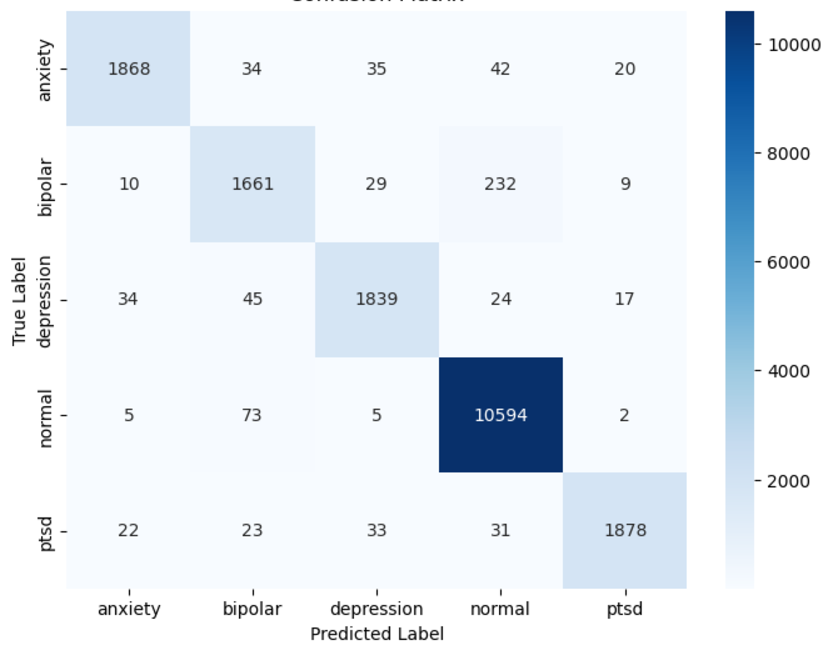
\includegraphics[width=\textwidth]{Images/EM CM.png}
        \caption*{Confusion Matrix (Ensemble Model 1)}
        \label{dfdl3123}  % Label for referencing the subfigure
    \end{subfigure}
    \hfill
    \begin{subfigure}[b]{0.47\textwidth}
        \centering
        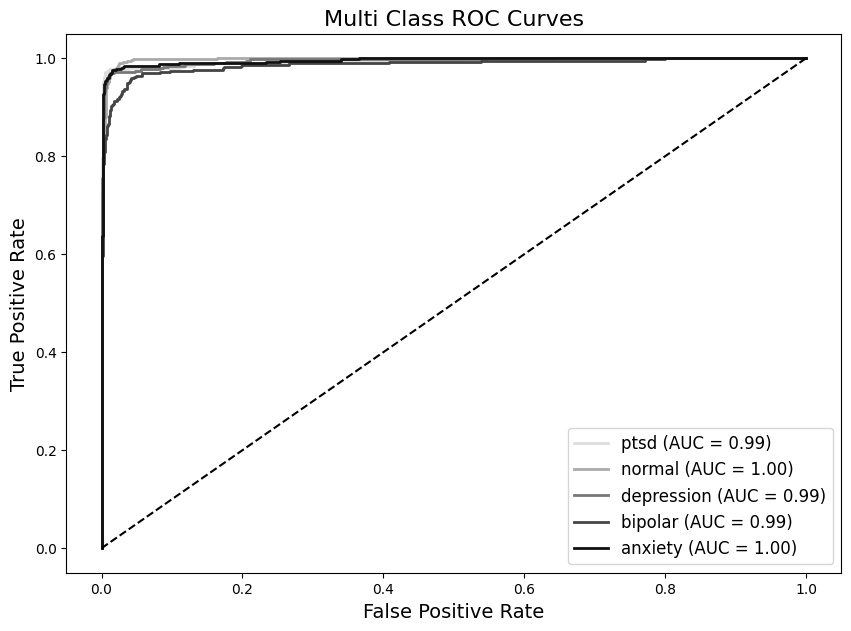
\includegraphics[width=\textwidth]{Images/EM ROC.png}
        \caption*{ROC AUC (Ensemble Model 1)}
        \label{dfdl12443}  % Label for referencing the subfigure
    \end{subfigure}
    \label{fig:ensemble_model_comparison}
\end{figure}

\vspace{-1em}

\begin{figure}[h!]
    \centering
    \begin{subfigure}[b]{0.47\textwidth}
        \centering
        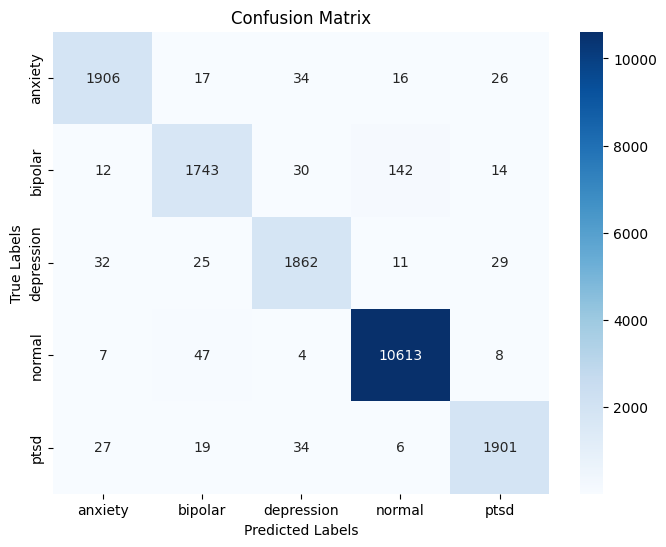
\includegraphics[width=\textwidth]{Images/EM2 CM.png}
        \caption*{Confusion Matrix (Ensemble Model 2)}
        \label{em2 cm}  % Label for referencing the subfigure
    \end{subfigure}
    \hfill
    \begin{subfigure}[b]{0.47\textwidth}
        \centering
        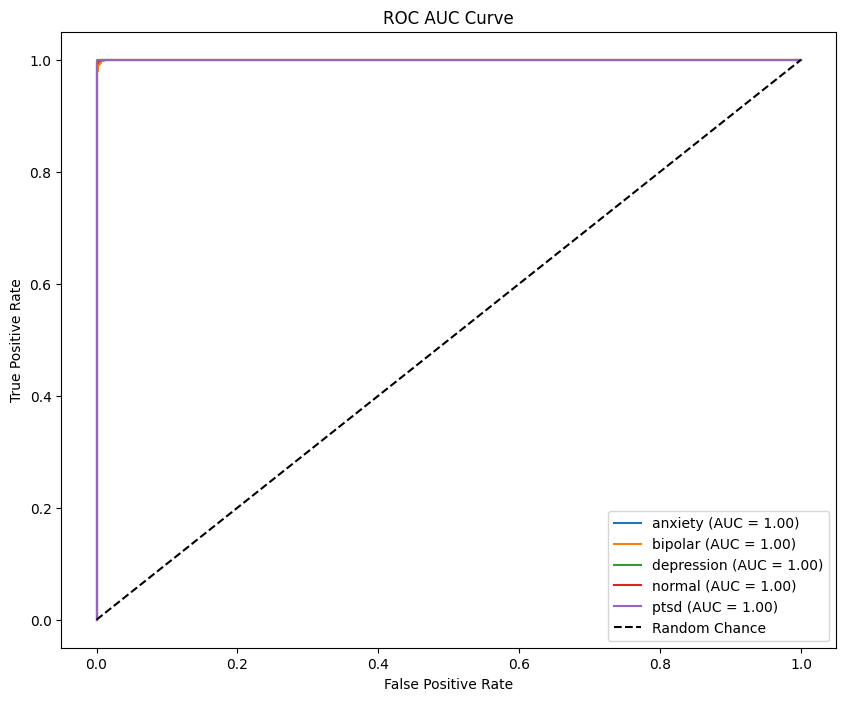
\includegraphics[width=\textwidth]{Images/EM2 ROC.png}
        \caption*{ROC AUC (Ensemble Model 2)}
        \label{em2 roc}  % Label for referencing the subfigure
    \end{subfigure}
    \label{fig:ensemble_model2_comparison}
\end{figure}

\vspace{-1em}

\begin{figure}[h!]
    \centering
    \begin{subfigure}[b]{0.47\textwidth}
        \centering
        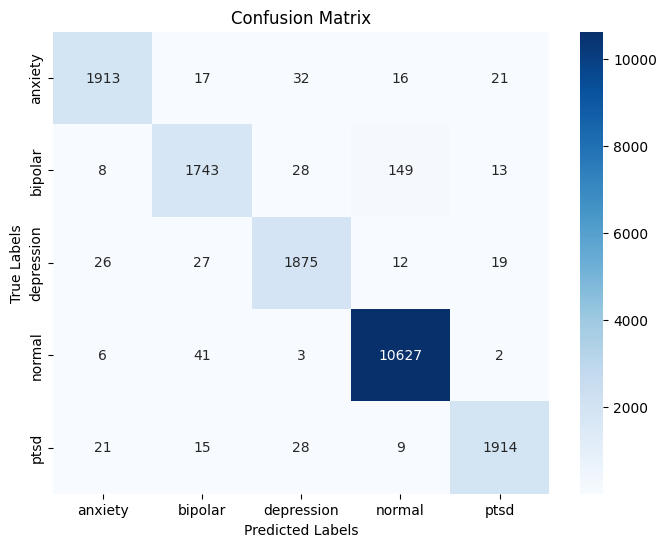
\includegraphics[width=\textwidth]{Images/EM3 CM.png}
        \caption*{Confusion Matrix (Ensemble Model 3)}
        \label{em3 cm}  % Label for referencing the subfigure
    \end{subfigure}
    \hfill
    \begin{subfigure}[b]{0.47\textwidth}
        \centering
        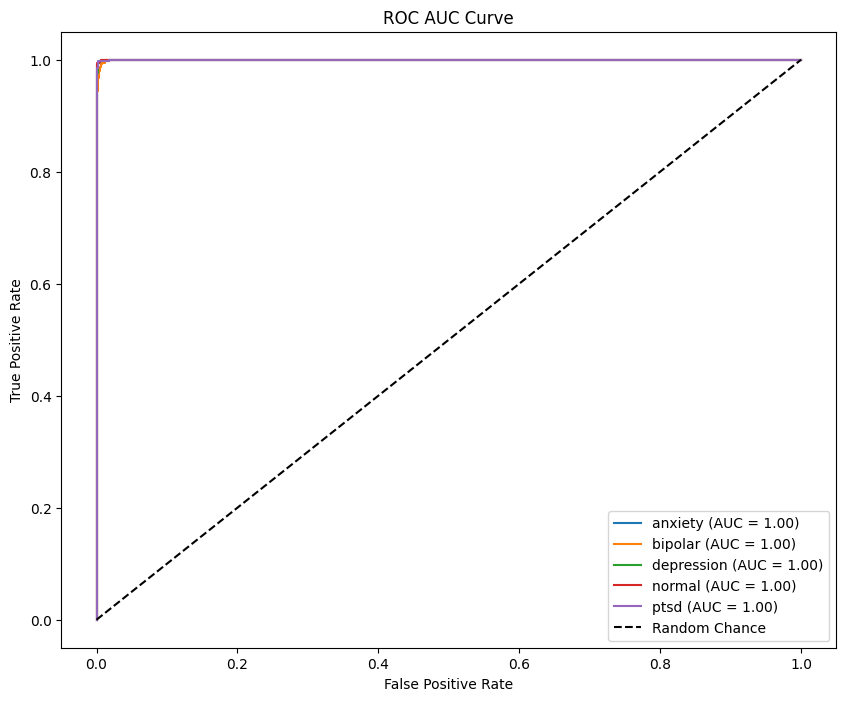
\includegraphics[width=\textwidth]{Images/EM3 ROC.png}
        \caption*{ROC AUC (Ensemble Model 3)}
        \label{em3 roc}  % Label for referencing the subfigure
    \end{subfigure}
    \label{fig:ensemble_model3_comparison}
\end{figure}

\pagebreak

\begin{figure}[h!]
    \centering
    \begin{subfigure}[b]{0.48\textwidth}
        \centering
        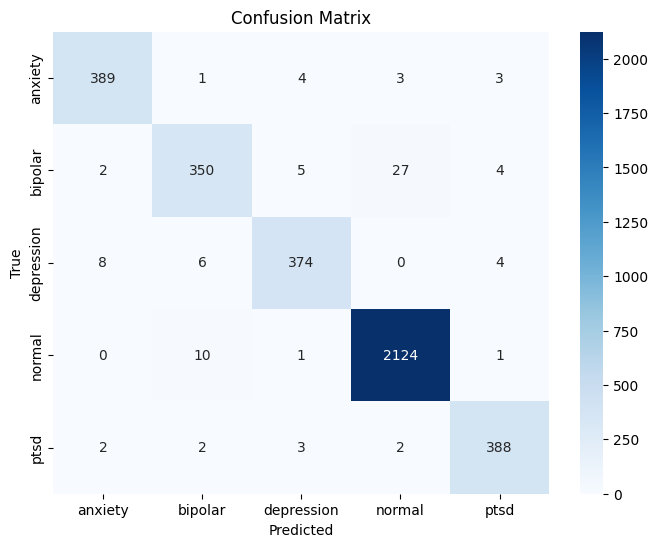
\includegraphics[width=\textwidth]{Images/BAG CM.png}
        \caption*{Confusion Matrix (Ensemble Model 4)}
        \label{bag cm}  % Label for referencing the subfigure
    \end{subfigure}
    \hfill
    \begin{subfigure}[b]{0.48\textwidth}
        \centering
        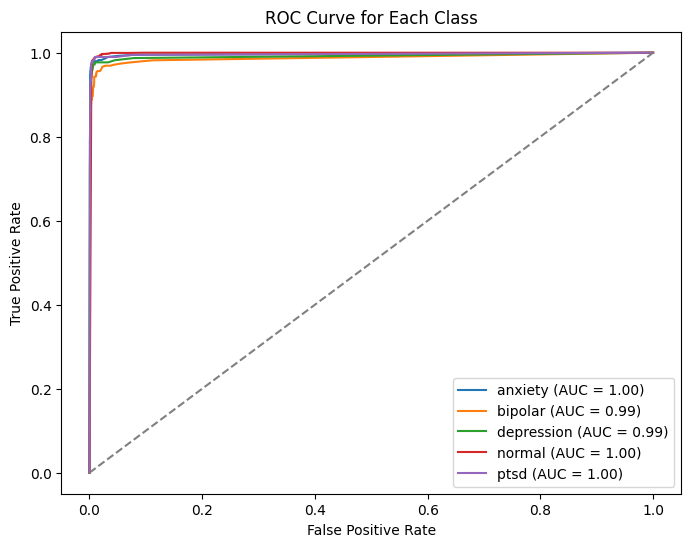
\includegraphics[width=\textwidth]{Images/BAG ROC.png}
        \caption*{ROC AUC (Ensemble Model 4)}
        \label{bag roc}  % Label for referencing the subfigure
    \end{subfigure}
    \label{fig:ensemble_model4_comparison}
\end{figure}


\begin{figure}[h!]
    \centering
    \begin{subfigure}[b]{0.48\textwidth}
        \centering
        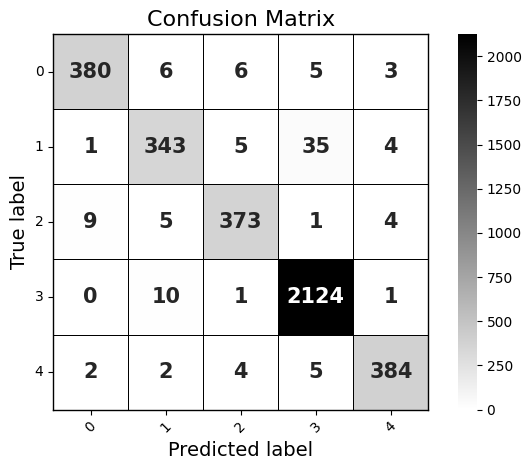
\includegraphics[width=\textwidth]{Images/BLD CM.png}
        \caption*{Confusion Matrix (Ensemble Model 5)}
        \label{bld cm}  % Label for referencing the subfigure
    \end{subfigure}
    \hfill
    \begin{subfigure}[b]{0.48\textwidth}
        \centering
        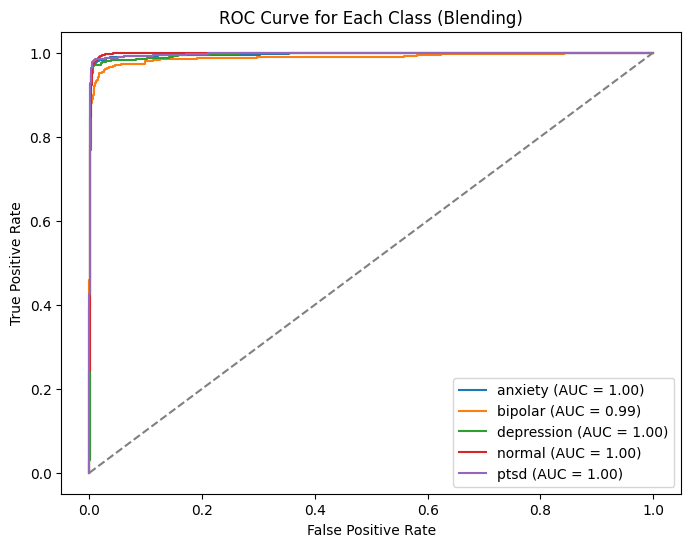
\includegraphics[width=\textwidth]{Images/BLD ROC.png}
        \caption*{ROC AUC (Ensemble Model 5)}
        \label{bld roc}  % Label for referencing the subfigure
    \end{subfigure}
    \label{fig:ensemble_model5_comparison}
\end{figure}


\begin{figure}[h!]
    \centering
    \begin{subfigure}[b]{0.48\textwidth}
        \centering
        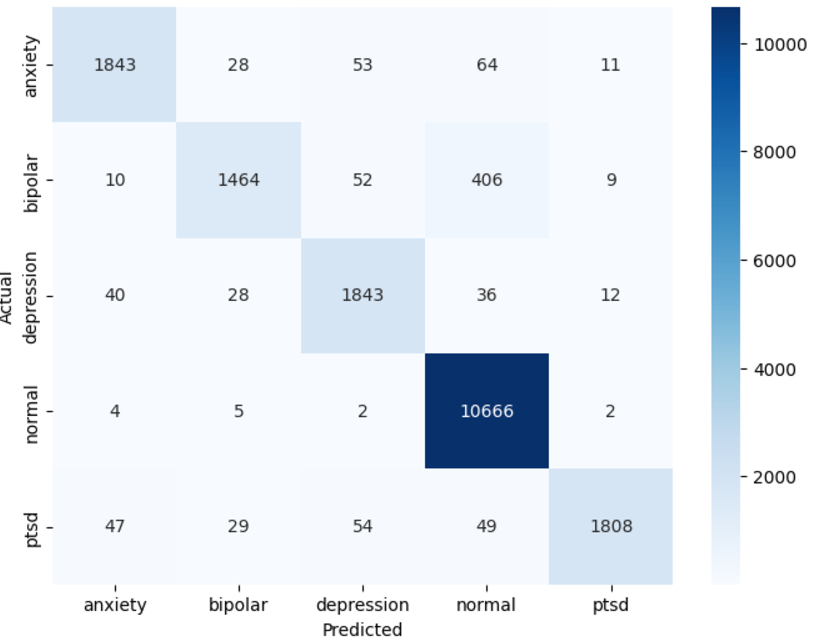
\includegraphics[width=\textwidth]{Images/WV CM.png}
        \caption*{Confusion Matrix (Ensemble Model 6)}
        \label{wv cm}  % Label for referencing the subfigure
    \end{subfigure}
    \hfill
    \begin{subfigure}[b]{0.48\textwidth}
        \centering
        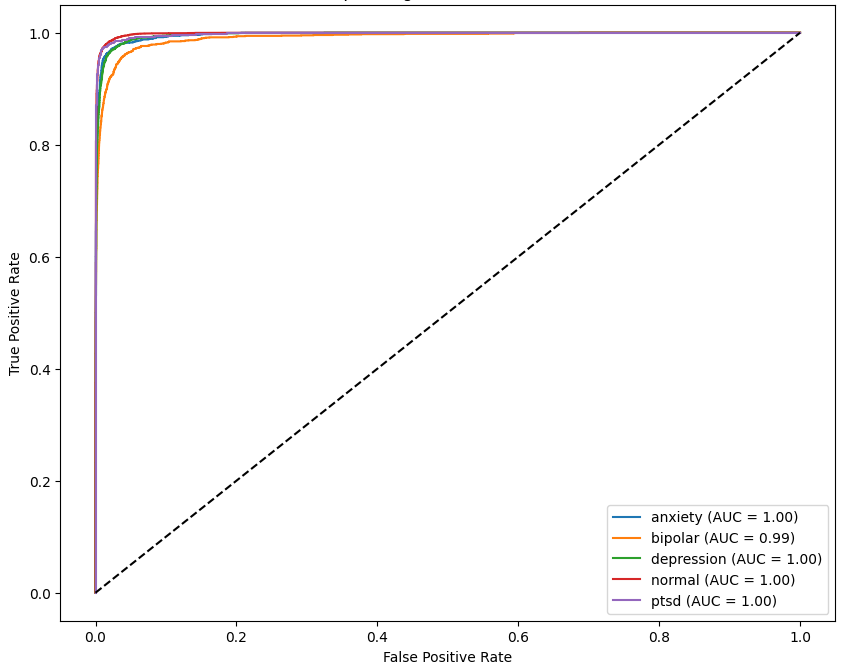
\includegraphics[width=\textwidth]{Images/WV ROC.png}
        \caption*{ROC AUC (Ensemble Model 6)}
        \label{wv roc}  % Label for referencing the subfigure
    \end{subfigure}
    \label{fig:ensemble_model6_comparison}
\end{figure}

\pagebreak

\begin{figure}[h!]
    \centering
    \begin{subfigure}[b]{0.48\textwidth}
        \centering
        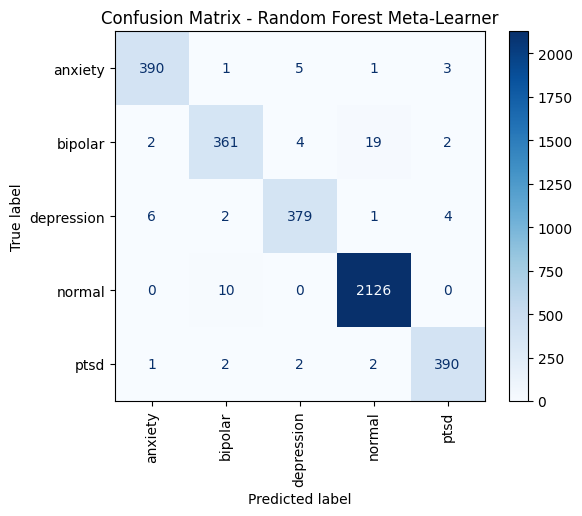
\includegraphics[width=\textwidth]{Images/EM T CM.png}
        \caption*{Confusion Matrix (Ensemble Model 7)}
        \label{em_t cm}  % Label for referencing the subfigure
    \end{subfigure}
    \hfill
    \begin{subfigure}[b]{0.48\textwidth}
        \centering
        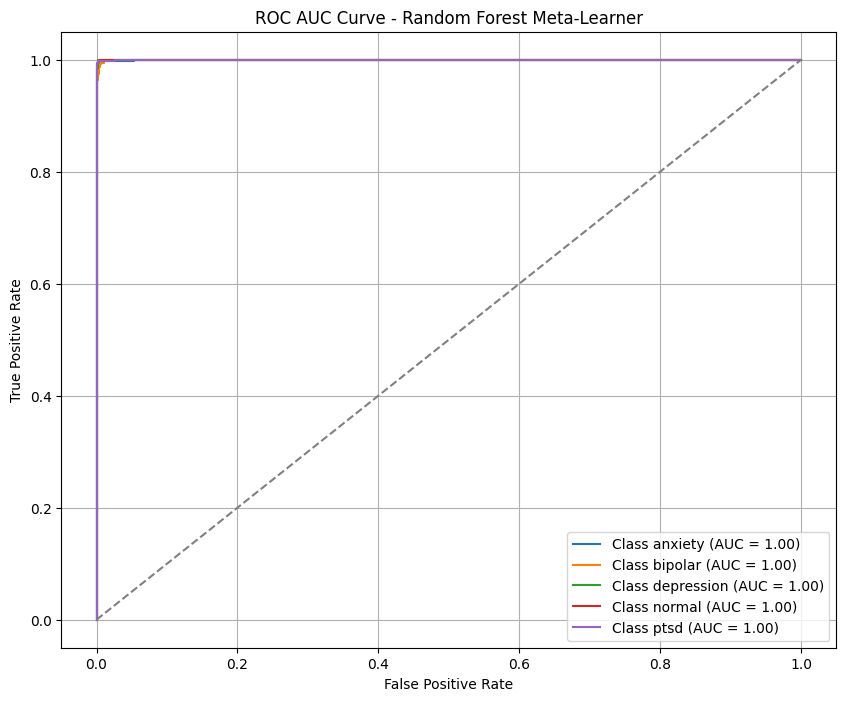
\includegraphics[width=\textwidth]{Images/EM T ROC.png}
        \caption*{ROC AUC (Ensemble Model 7)}
        \label{em_t roc}  % Label for referencing the subfigure
    \end{subfigure}
    \label{fig:ensemble_model7_comparison}
\end{figure}

\begin{figure}[h!]  
    \centering
    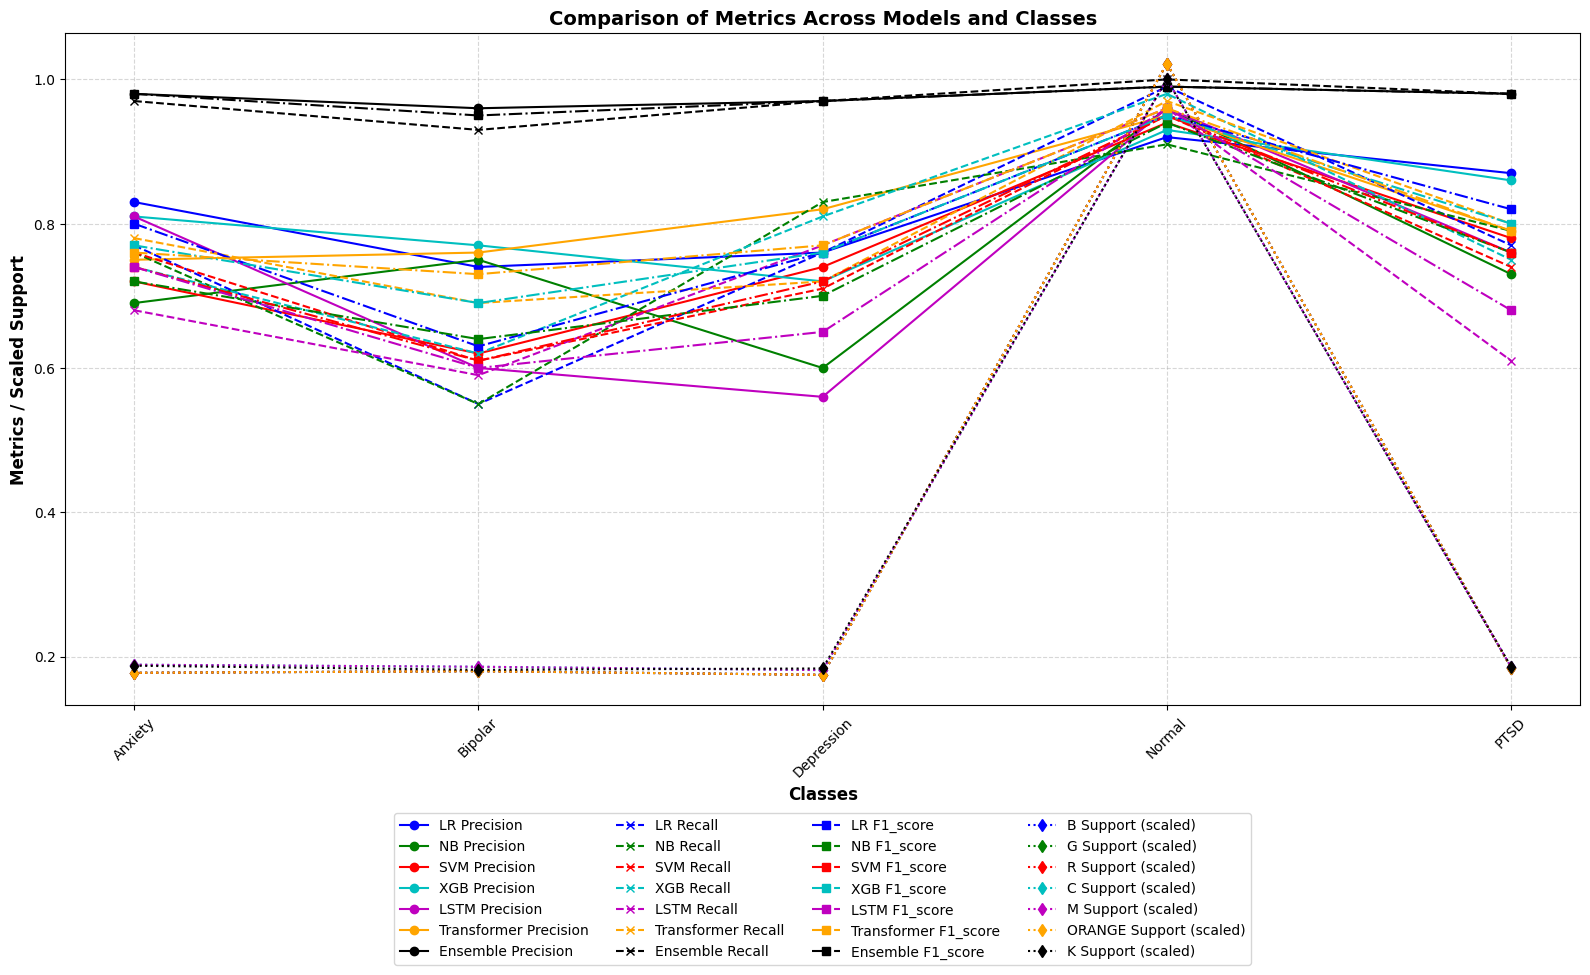
\includegraphics[width=0.8\textwidth]{Images/EM T RESULT.png}  
    \caption*{Comparison of Base Models and Ensemble Model7}
    \label{lstm arch}  % Label for referencing the figure
\end{figure}

\begin{table}[H]
    \centering
    \caption*{Comparison of all the 7 Ensemble Models}
    \label{tab:ensemble_comparison}
    \begin{tabularx}{\textwidth}{|l|c|X|X|X|}
    \hline
    \textbf{Model} & \textbf{Accuracy} & \textbf{Key Components} & \textbf{Advantages} & \textbf{Limitations} \\
    \hline
    Ensemble Model 1 & 96.08\% & Logistic Regression + XGBoost & Balanced performance (e.g., Anxiety: Prec=0.97, Rec=0.94, F1=0.95); robust macro/weighted averages & May not fully capture complex, non-linear, context-dependent patterns \\
    \hline
\end{tabularx}
\end{table}

\pagebreak

\begin{table}[H]
    \centering
    \caption*{Comparison of all the 7 Ensemble Models}
    \label{tab:ensemble_comparison}
    \begin{tabularx}{\textwidth}{|l|c|X|X|X|}
    \hline
    \textbf{Model} & \textbf{Accuracy} & \textbf{Key Components} & \textbf{Advantages} & \textbf{Limitations} \\
    \hline
    Ensemble Model 2 & 97.93 & XGBoost as meta-learner combining base models (LR, SVM, NB, LSTM) & Near-perfect ROC AUC (1.0 for Anxiety, Normal, PTSD; 0.99 for Bipolar, Depression); effective handling of imbalanced data & Potential overfitting if base model predictions are highly correlated \\
    \hline
    Ensemble Model 3 & 97.76 & Random Forest used as meta-learner & High overall accuracy with very few misclassifications; robust due to bootstrapping and random feature selection & Slightly lower recall in some classes (e.g., Bipolar) \\
    \hline
    Ensemble Model 4 & 97.63\% & Bagging classifier (similar to Random Forest) & Excellent performance with near-perfect results for the “Normal” class & Tendency to overfit due to using all features without feature-level randomness \\
    \hline
    Ensemble Model 5 & 97.17\% & Blending Meta-Learner trained directly on base model predictions & Strong precision, recall, and F1-scores across classes; stable cross-validation performance & More prone to overfitting compared to stacking ensembles (e.g., with a Random Forest meta-learner) \\
    \hline
    Ensemble Model 6 & 95.15\% & Weighted Voting ensemble combining base model outputs & Solid overall performance with high recall for “Normal” and computational efficiency & Lacks optimal inter-model learning; struggles with distinguishing bipolar disorder \\
    \hline
    Ensemble Model 7 & 98.03\% & Transformer-based model (base) + meta-learner (Random Forest and others) & Near-perfect ROC AUC (1.0 across classes); excellent accuracy and robust classification & Increased computational complexity due to Transformer integration \\
    \hline
    \end{tabularx}
\end{table}


\pagebreak

\noindent
Below is a comparison of all the ensemble models for reference

\begin{figure}[h!]  
    \centering
    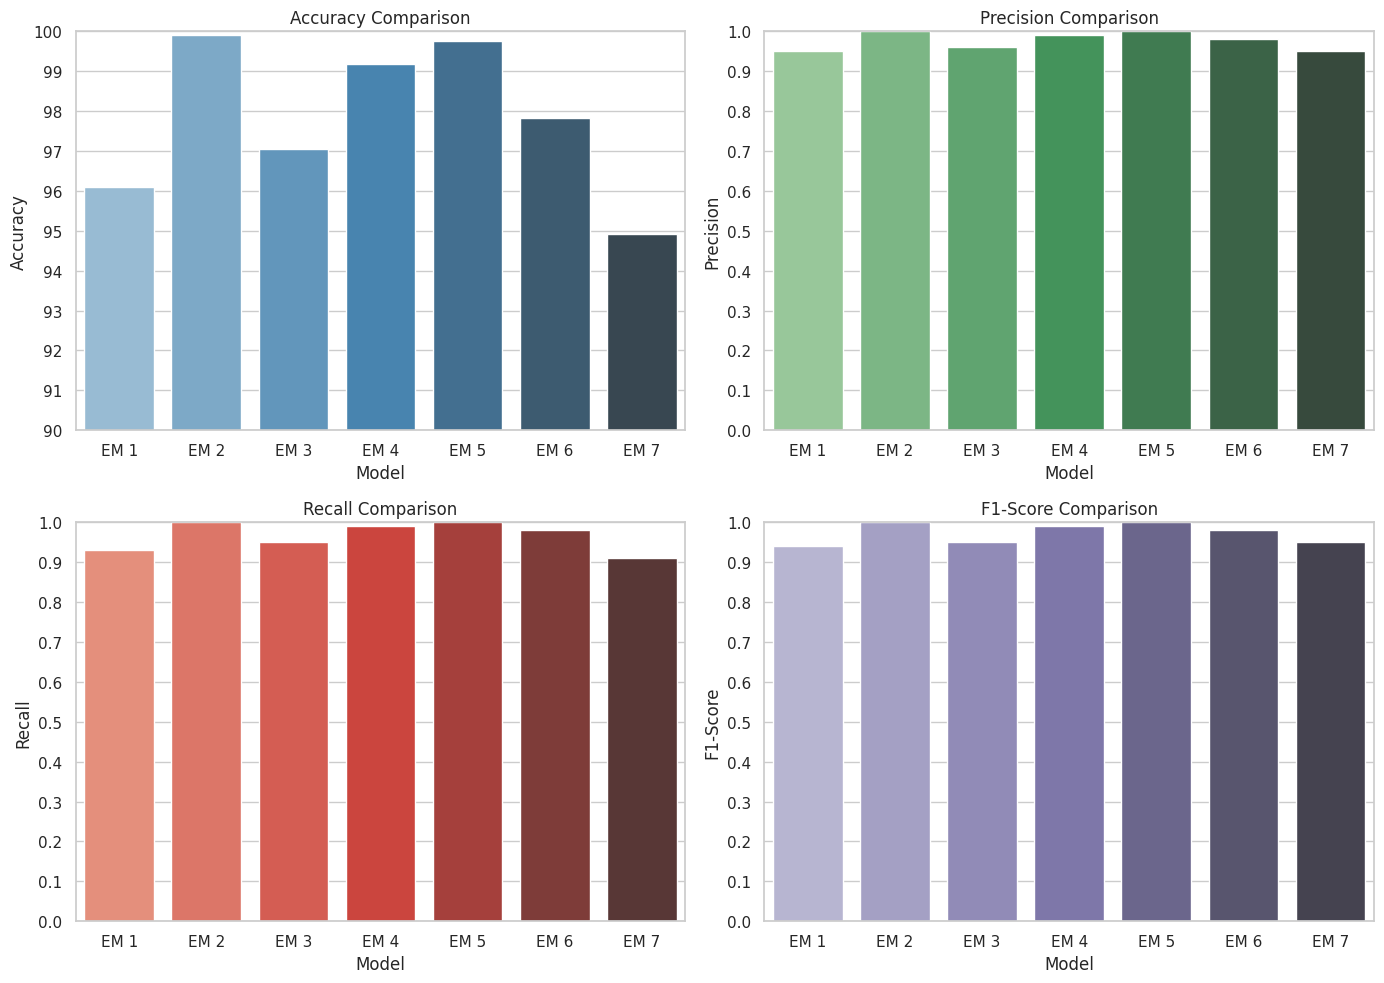
\includegraphics[width=1.0\textwidth]{Images/EM COMPARE.png}  
    \caption*{Comparison of all Ensemble Models}
    \label{lstm arch}  % Label for referencing the figure
\end{figure}



\subsection{Results from hierarchical Ensemble Models}

\noindent
Ensemble Model 7 is applied on different subsets of a very large dataset to create hierarchical ensemble models. The performance of each model is evaluated, and the results are compared to the global ensemble model. 

\begin{center}
    \textbf{Performance Comparison of Models} \\[0.5em]
    % Resize the table to fit the text width
    \resizebox{\textwidth}{!}{%
    \begin{tabular}{|c|c|c|c|c|c|c|c|}
        \hline
        \textbf{Model} & \textbf{Subset 1} & \textbf{Subset 2} & \textbf{Subset 3} & \textbf{Subset 4} & \textbf{Subset 5} & \textbf{Subset 6} & \textbf{ENSEMBLE} \\ \hline
        Logistic Regression & 87.66 & 85.07 & 86.74 & 90.61 & 88.17 & 72.62 & \textbf{90.90} \\ \hline
        Naive Bayes         & 83.63 & 81.71 & 83.50 & 84.44 & 85.93 & 64.33 & \textbf{84.15} \\ \hline
        SVM                 & 85.13 & 82.30 & 83.50 & 88.34 & 85.45 & 67.81 & \textbf{91.79} \\ \hline
        XGBoost             & 87.39 & 85.79 & 86.78 & 91.37 & 86.32 & 70.95 & \textbf{67.67} \\ \hline
        LSTM                & 84.91 & 81.63 & 81.83 & 87.22 & 85.38 & 67.74 & \textbf{87.48} \\ \hline
        Transformer         & 88.50 & 84.50 & 86.50 & 89.35 & 87.62 & 72.40 & \textbf{91.53} \\ \hline
        \textbf{ENSEMBLE}   & \textbf{98.03} & \textbf{94.85} & \textbf{96.96} & \textbf{97.79} & \textbf{96.86} & \textbf{92.57} & 
        \diagbox[height=2em,width=7em]%
        {\makebox[2.5em][r]{\textbf{96.24}}}%
        {\makebox[2.5em][l]{\textbf{96.25}}} \\ \hline
    \end{tabular}
    } % End of resizebox
    \\[1em]
    \textbf{Note:} The final ensemble models from two different architectures achieved accuracies of \textbf{96.24\%} and \textbf{96.25\%} respectively.
\end{center}

\pagebreak

\begin{figure}[h!]  
    \centering
    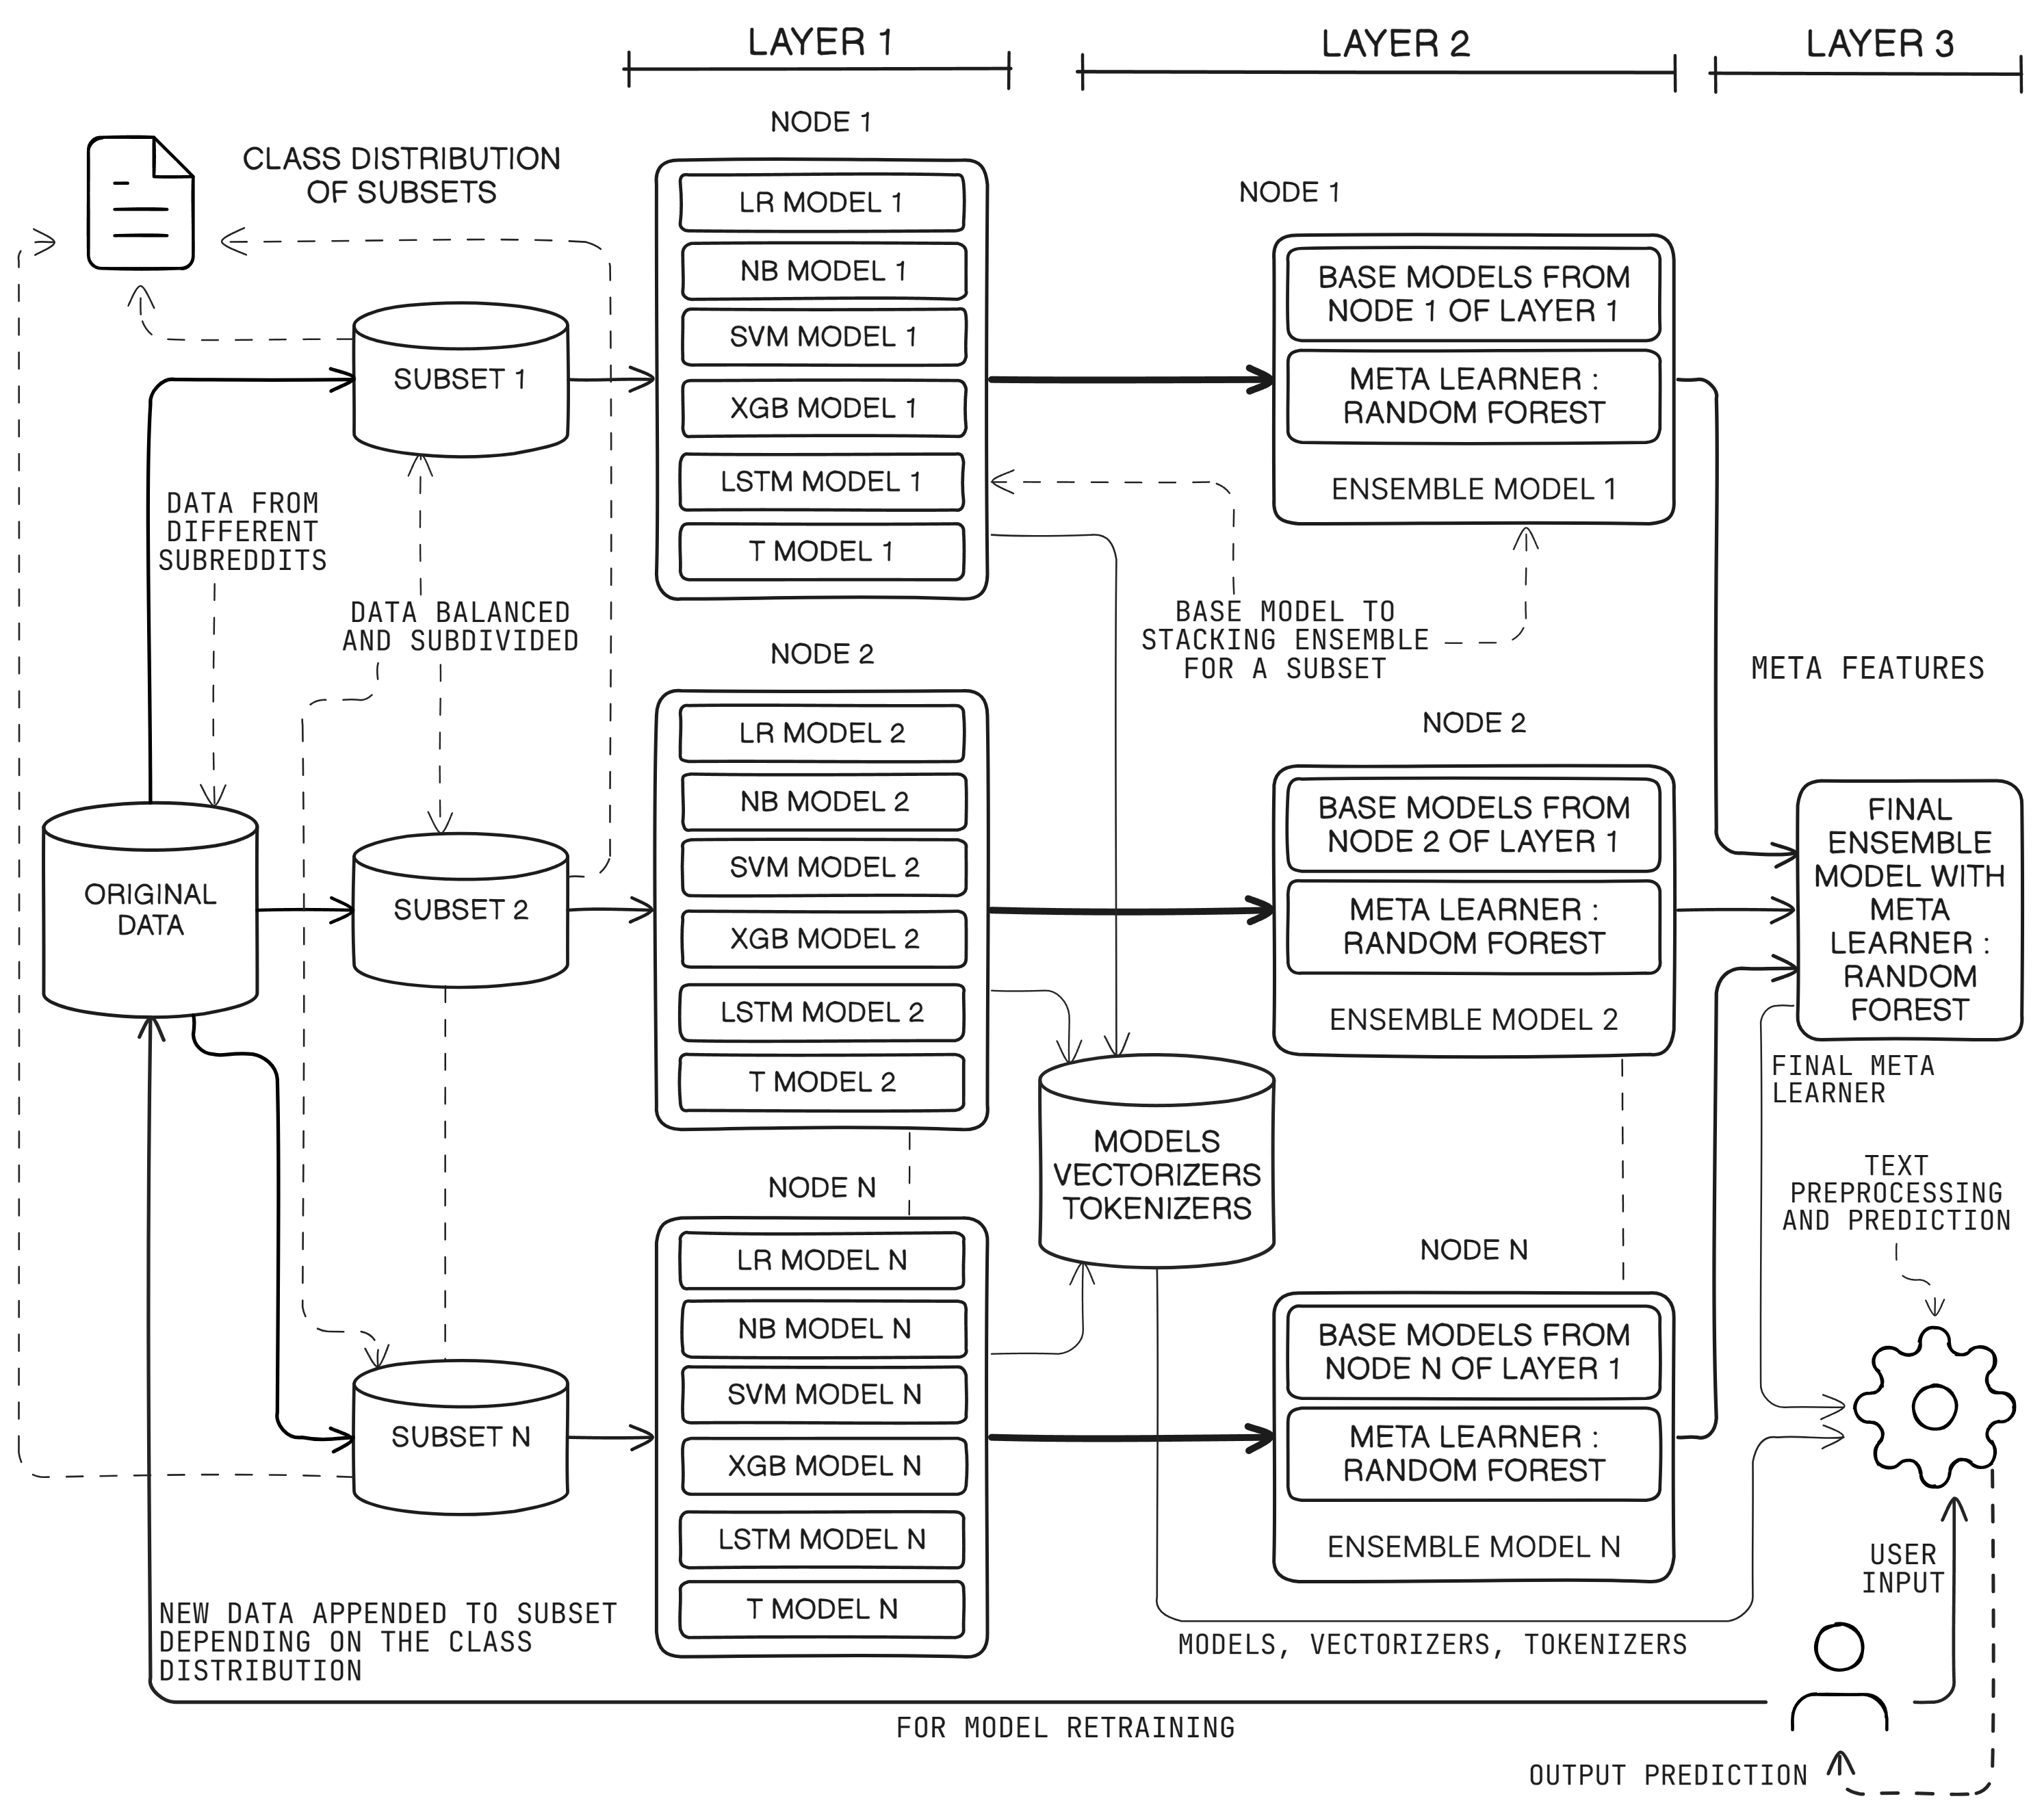
\includegraphics[width=0.9\textwidth]{Images/Distributed.png}  
    \caption*{Scalable Distributed Architecture 1}
    \label{lstm archi}  % Label for referencing the figure
\end{figure}

\begin{table}[H]
    \caption*{Summary of Architecture 1: Hierarchical Ensemble}
    \label{tab:arch1}
    \begin{tabularx}{\textwidth}{|p{3cm}|X|}
    \hline
    \textbf{Aspect} & \textbf{Description} \\ \hline
    Data Partitioning & The dataset is divided into manageable subsets for independent processing. \\ \hline
    Base Models & Each subset trains base models (Logistic Regression, Naive Bayes, SVM, LSTM, XGBoost, and Custom Transformers). \\ \hline
    Subset Ensemble & For each subset, a Random Forest meta learner is used to combine the base models into a subset-specific ensemble. \\ \hline
    Global Aggregation & The subset-specific ensembles are aggregated to form a final global ensemble, capturing comprehensive learning. \\ \hline
    Scalability & Designed for distributed processing; subsets can be processed in parallel across multiple nodes. \\ \hline
    Fault Tolerance & Modular design ensures that failure in one subset does not impact the overall ensemble performance. \\ \hline
    Distributed Processing & Worker nodes independently train base models and report to a central controller that aggregates the results. \\ \hline
    \end{tabularx}
\end{table}
    
\pagebreak

\begin{figure}[h!]  
    \centering
    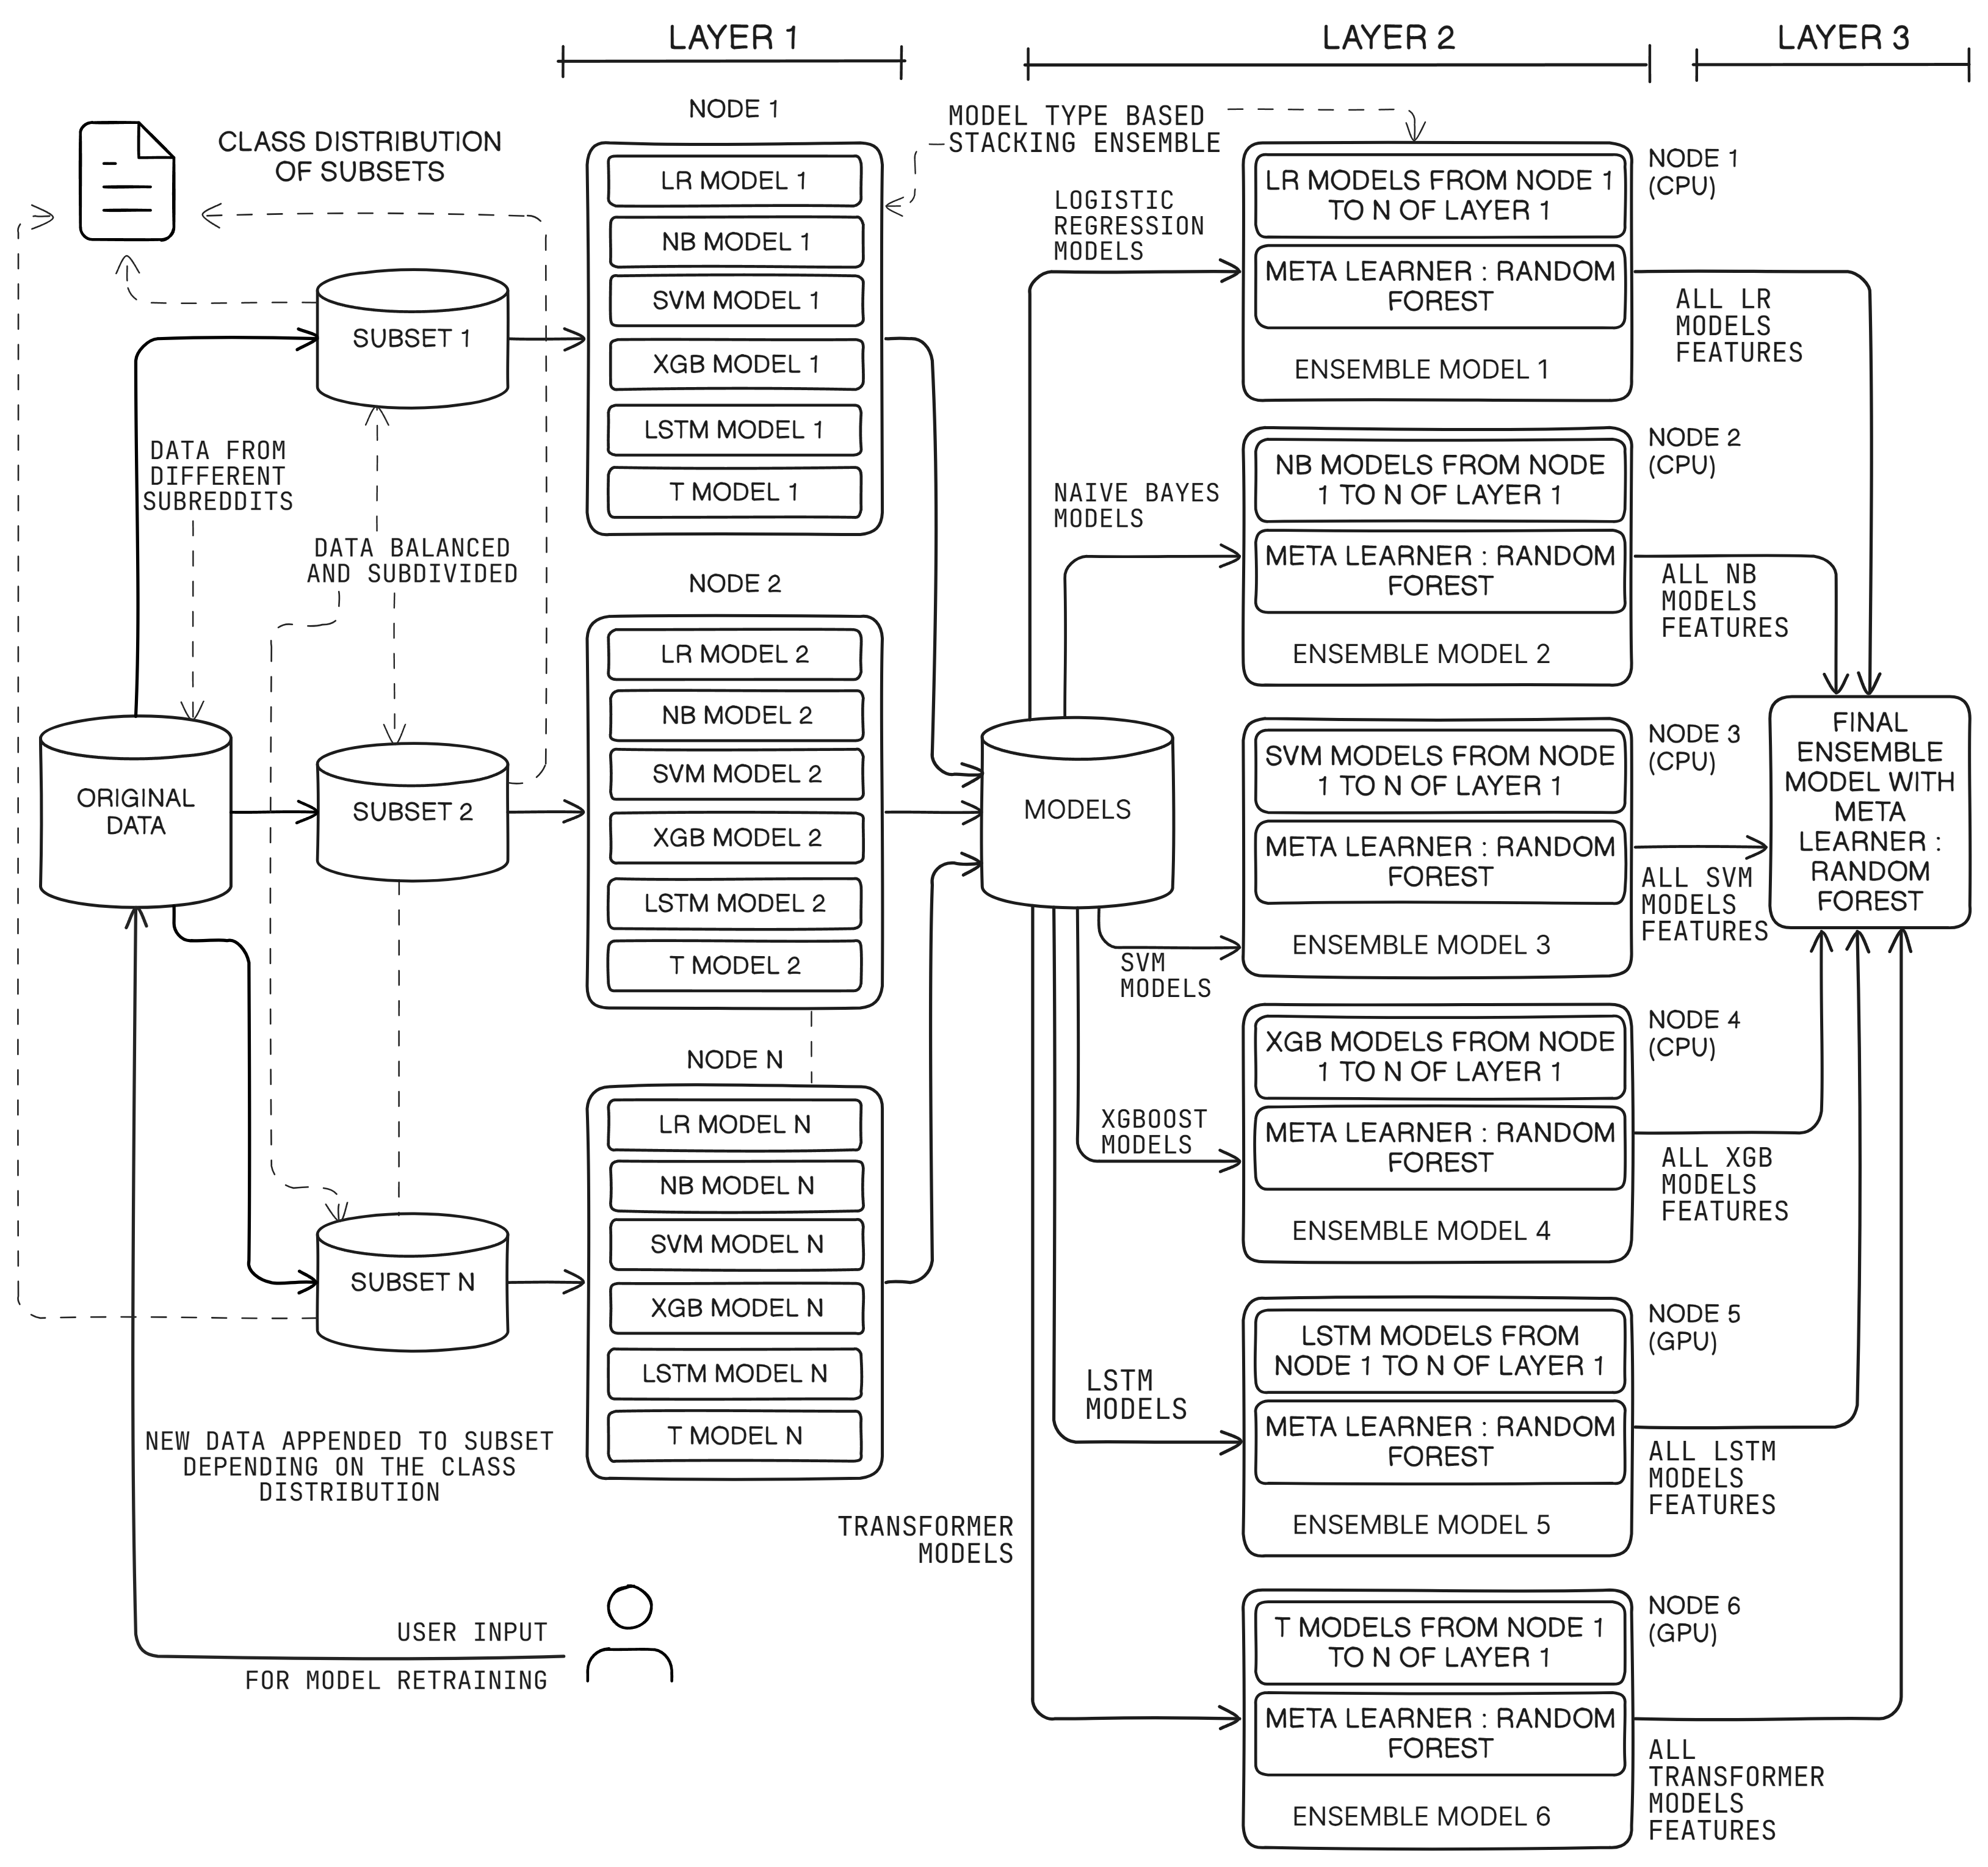
\includegraphics[width=0.82\textwidth]{Images/Distributed2.png}  
    \caption*{Scalable Distributed Architecture 2}
    \label{lstm archi}  % Label for referencing the figure
\end{figure}

\begin{table}[H]
    \caption*{Summary of Architecture 2: Optimized Hierarchical Ensemble}
    \label{tab:arch2}
    \begin{tabularx}{\textwidth}{|p{3cm}|X|}
    \hline
    \textbf{Aspect} & \textbf{Description} \\ \hline
    Optimized Aggregation & Models of the same type from all subsets are combined into a single intermediate ensemble for that model type. \\ \hline
    Intermediate Ensembles & Produces six intermediate ensembles (one each for Logistic Regression, Naive Bayes, SVM, XGBoost, LSTM, and Transformer). \\ \hline
    Final Ensemble & The six intermediate ensembles are aggregated via a meta learner (Random Forest) to form the final ensemble. \\ \hline
    Fixed Ensemble Count & The number of intermediate ensembles is fixed at six, regardless of the number of subsets, reducing computational overhead. \\ \hline
    Efficient Resource Utilization & GPUs are reserved for training the computationally intensive LSTM and Transformer ensembles; lightweight meta learners (e.g., Logistic Regression or Random Forest) optimize aggregation. \\ \hline
    Data Bus Implementation & A structured data bus efficiently transfers models from subsets to intermediate nodes, reducing latency and synchronization overhead. \\ \hline
    Improved Cross-Validation & Streamlined aggregation minimizes redundancy, resulting in faster cross-validation and training on large datasets. \\ \hline
    \end{tabularx}
\end{table}
    

\pagebreak

\noindent
To determine \( n \), the number of subsets, based on the size of the original dataset, it is crucial to consider computational efficiency, memory constraints, and sequential execution. Given that the dataset has \( D = 167,229 \) records and is processed sequentially in Google Colab with 12GB of RAM per node, the number of subsets \( n \) must strike a balance between memory usage and model performance. In this case, you chose \( n = 6 \) subsets, which implies a subset size \( S \) of:

\[
S = \frac{D}{n} = \frac{167,229}{6} \approx 27,872 \, \text{records per subset}.
\]

\vspace{1em}

\noindent
The choice of \( n = 6 \) is reasonable given the following factors:

\vspace{1em}

\noindent
1. \textbf{Memory Constraints}: Google Colab provides 12GB of RAM. Each subset must fit within this memory while accommodating the model's requirements for training and validation. Processing approximately 27,833 records at a time is well-suited to this memory limit for most machine learning models, including Logistic Regression, SVM, LSTM, and Transformer-based models.

\noindent
2. \textbf{Sequential Execution}: Since the architectures are implemented sequentially, the number of subsets \( n \) does not need to align with the number of computational nodes. Instead, the goal is to divide the dataset into manageable chunks that reduce training time and memory overhead for each subset.

\noindent
3. \textbf{Performance and Aggregation}: With \( n = 6 \), both architectures remain computationally feasible. In Architecture 1, \( n = 6 \) leads to six independent intermediate ensemble models, which are aggregated into the final ensemble. In Architecture 2, models of the same type from all six subsets are combined into six intermediate ensemble models, one for each type of algorithm.

\vspace{1em}

\noindent
The web application uses only the model from the first intermediate node of Architecture 1, as retraining the larger dataset model takes over 20 minutes.

% \vspace{1em}

\subsection{User Interface of the Application}

\noindent
Below are some snapshots from the web application.

\begin{figure}[H]  
    \centering
    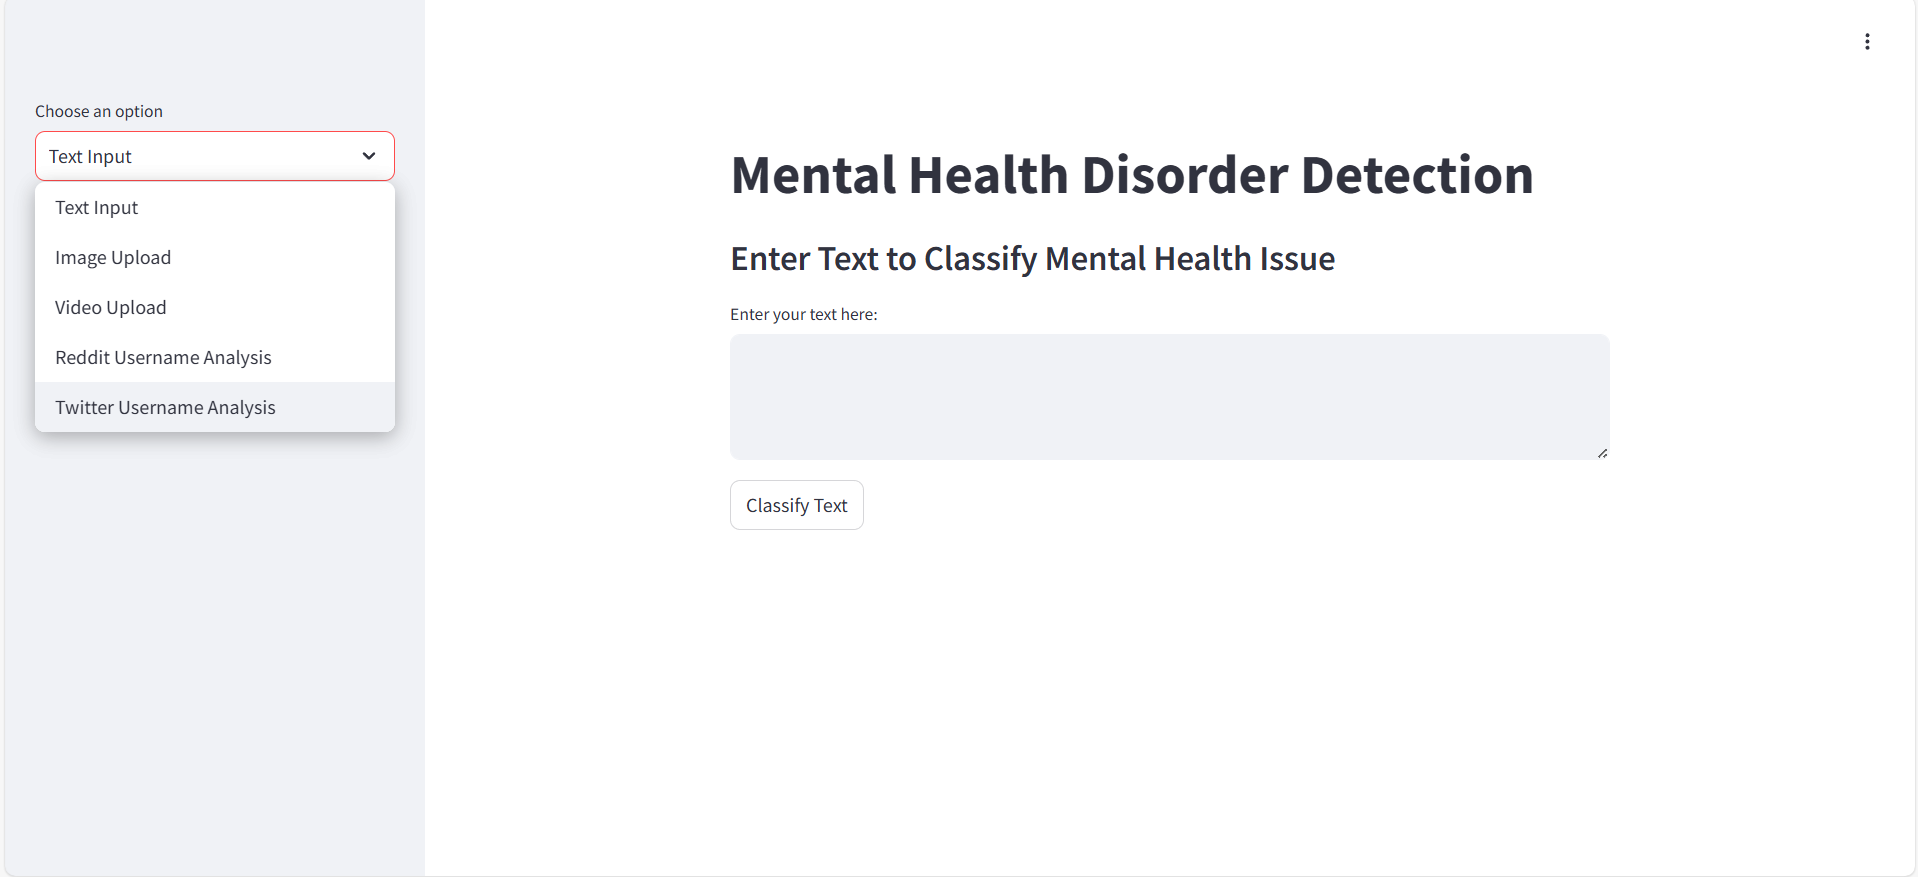
\includegraphics[width=0.7\textwidth]{App Images/01 Interface.png}  
    \caption*{List of Options for the User}
    \label{01i}  % Label for referencing the figure
\end{figure}


\pagebreak

\begin{figure}[h!]
    \centering
    % First subfigure: Text Input Option
    \begin{subfigure}[b]{0.495\textwidth}
        \centering
        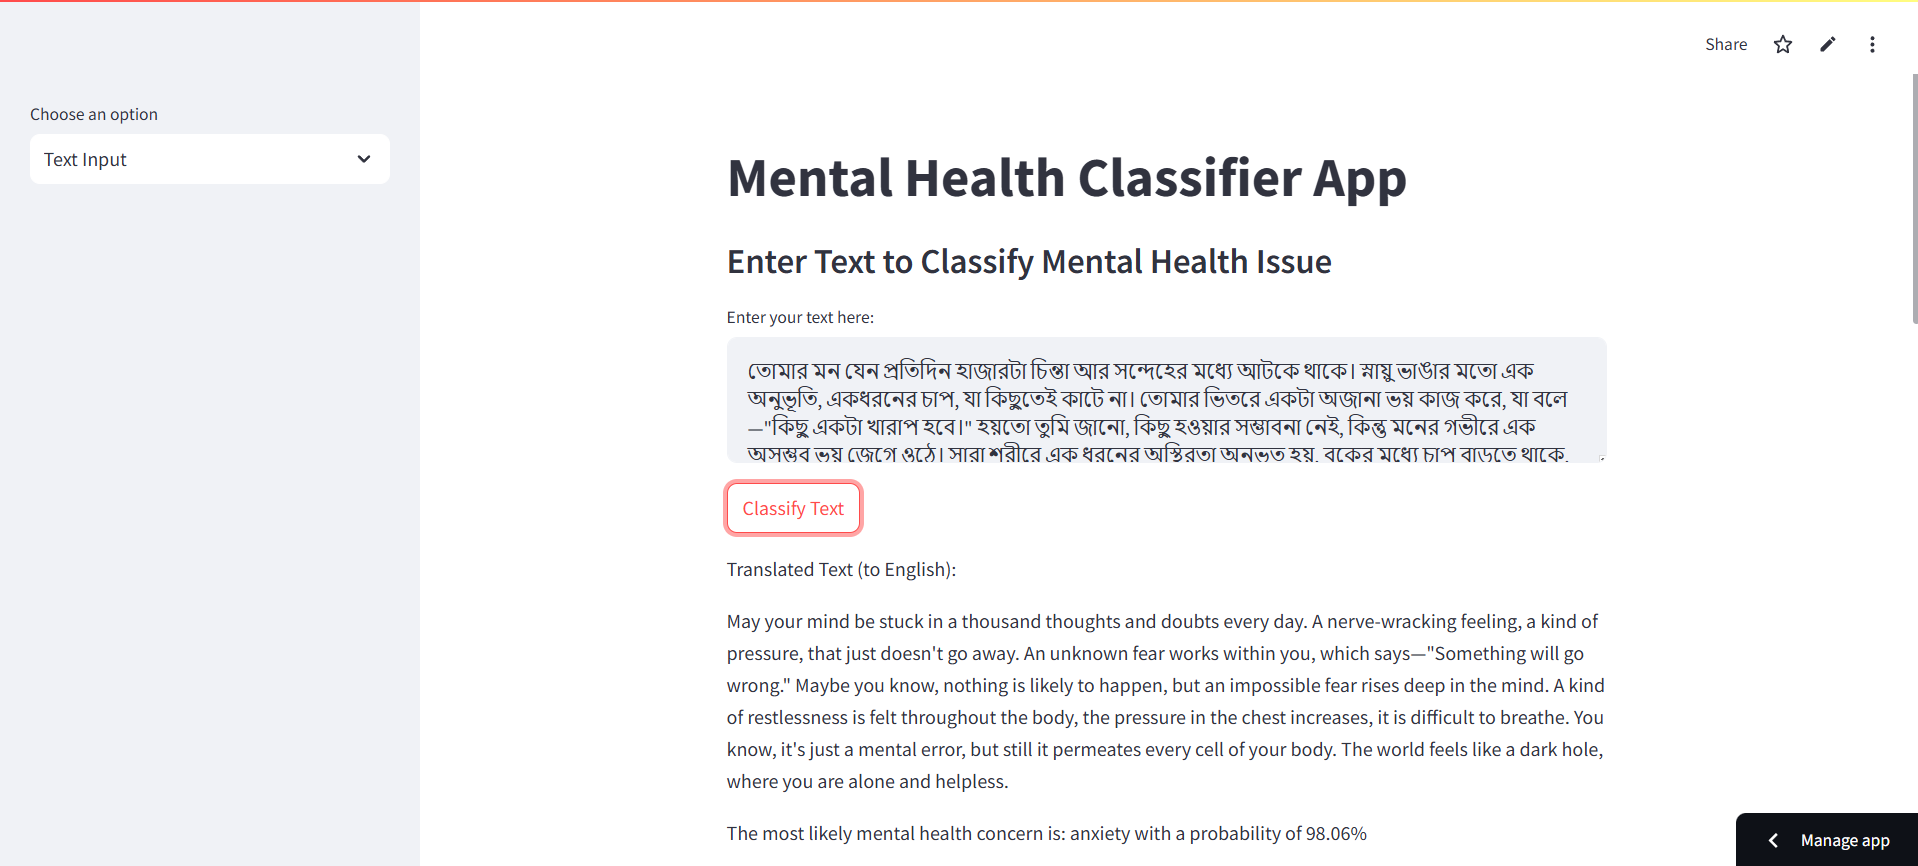
\includegraphics[width=\textwidth]{App Images/02 Interface.png}
        \caption*{Text Input Option}
        \label{fig:02i}
    \end{subfigure}
    \hfill
    % Second subfigure: Upload Image
    \begin{subfigure}[b]{0.495\textwidth}
        \centering
        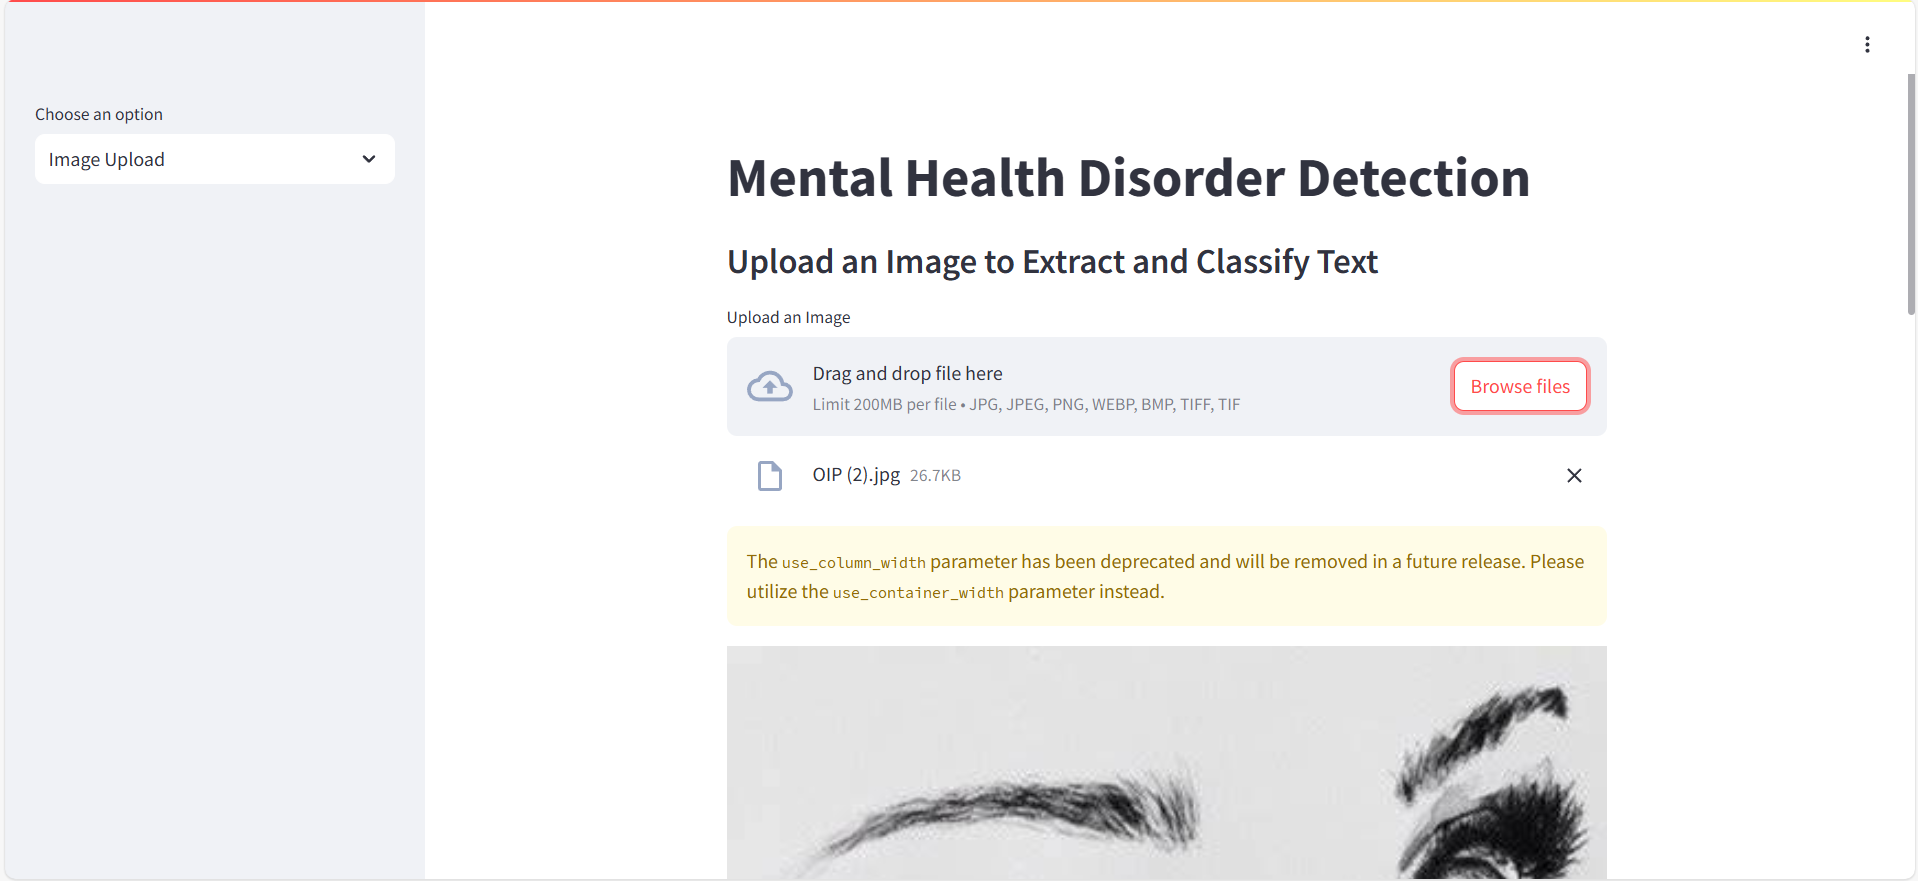
\includegraphics[width=\textwidth]{App Images/04 Interface.png}
        \caption*{Upload Image Option}
        \label{fig:04i}
    \end{subfigure}
    \label{fig:app_interfaces}
\end{figure}

\vspace{-2em}

\begin{figure}[h!]
    \centering
    % First subfigure: Upload Video
    \begin{subfigure}[b]{0.495\textwidth}
        \centering
        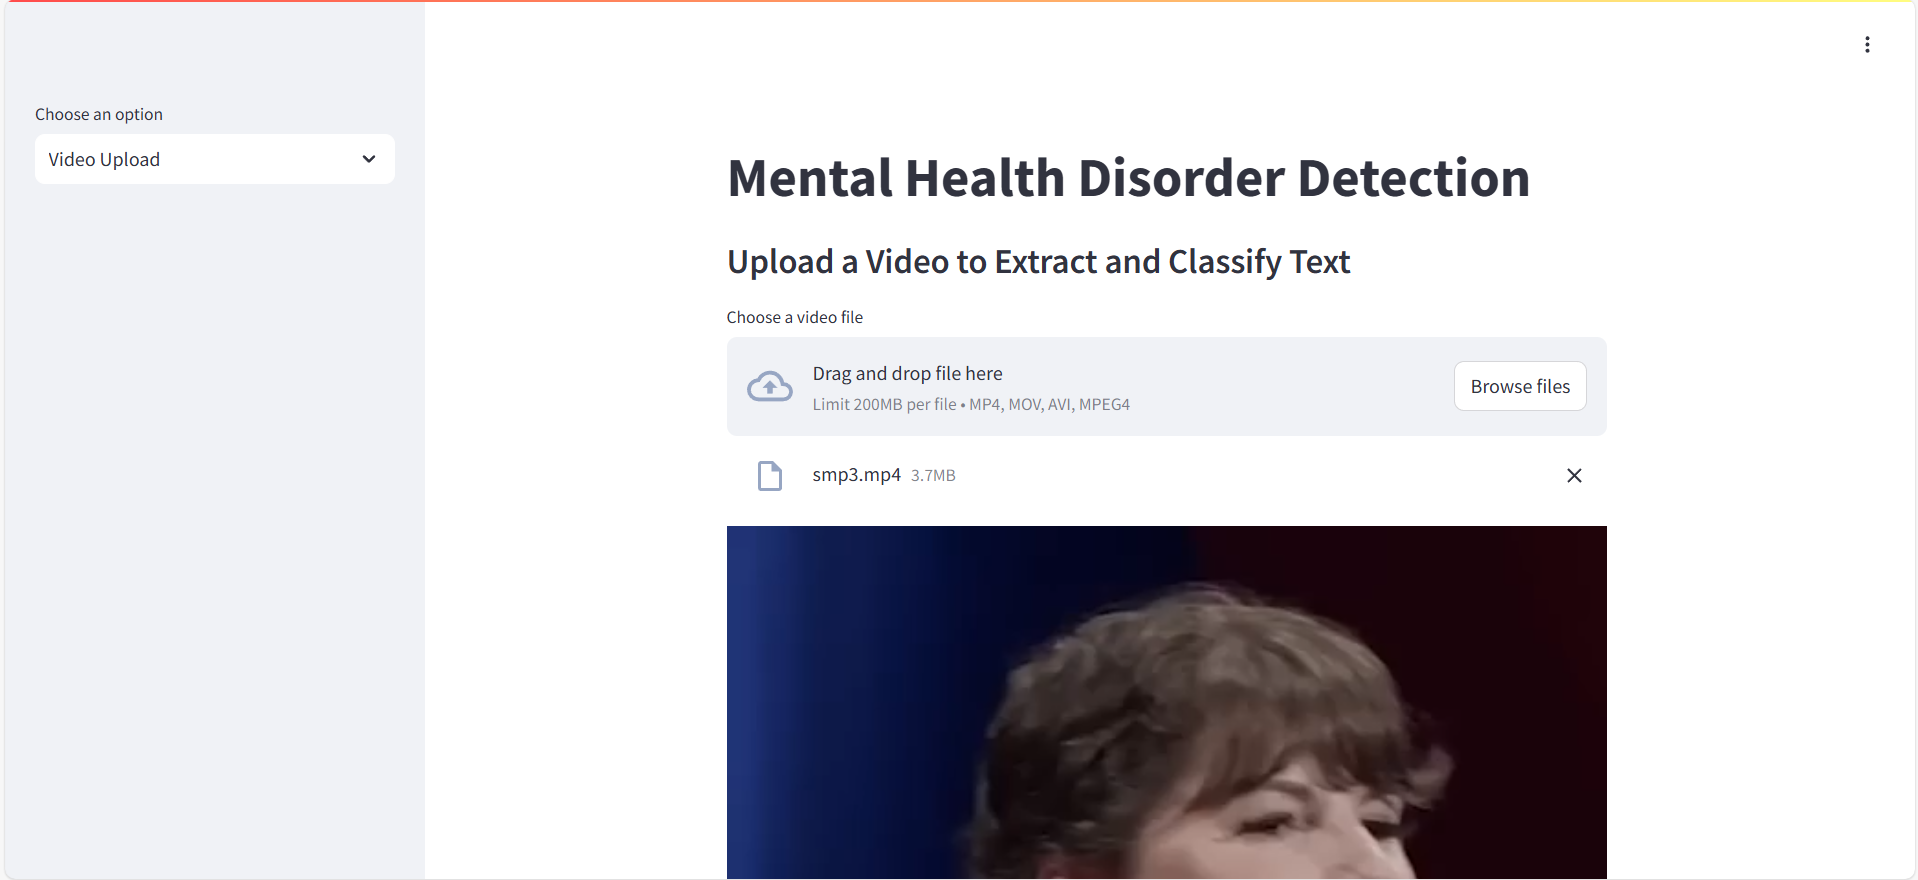
\includegraphics[width=\textwidth]{App Images/12 Interface.png}
        \caption*{Upload Video Option}
        \label{fig:06i4}
    \end{subfigure}
    \hfill
    % Second subfigure: PDF Upload Option
    \begin{subfigure}[b]{0.495\textwidth}
        \centering
        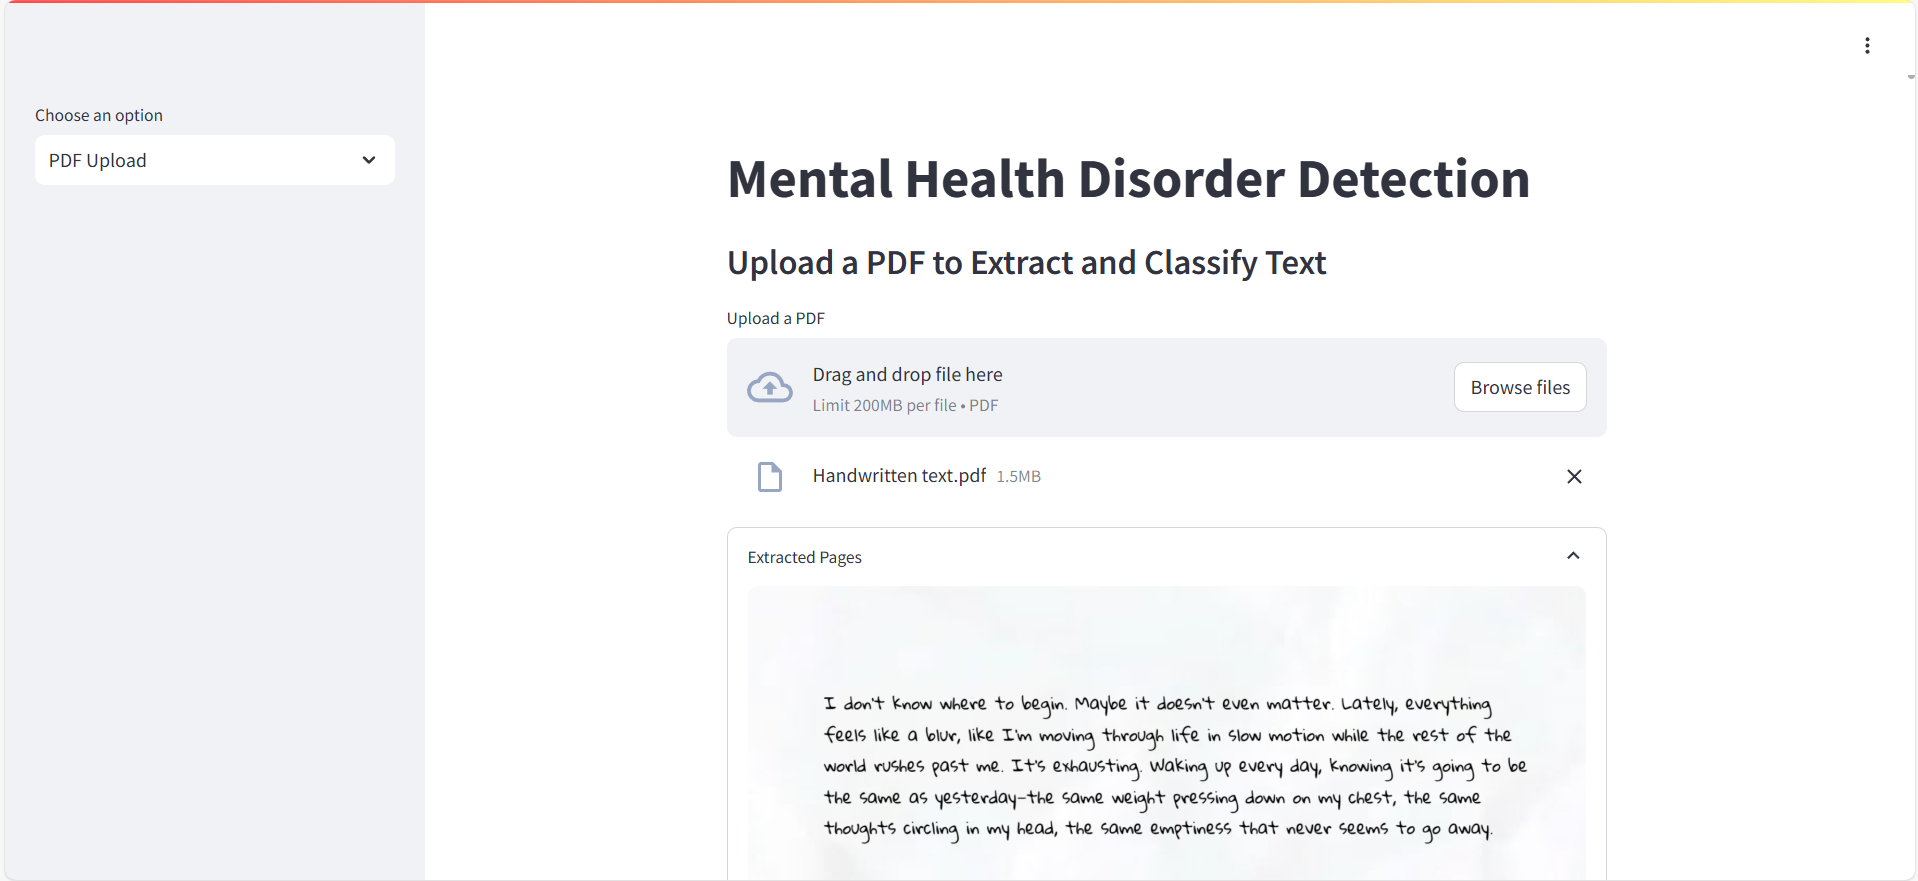
\includegraphics[width=\textwidth]{App Images/20 Interface.png}
        \caption*{PDF Upload Option}
        \label{fig:10i23445}
    \end{subfigure}
    \label{fig:app_interfaces_upload}
\end{figure}

\vspace{-2em}

\begin{figure}[h!]
    \centering
    % First subfigure: User response to Image Option
    \begin{subfigure}[b]{0.495\textwidth}
        \centering
        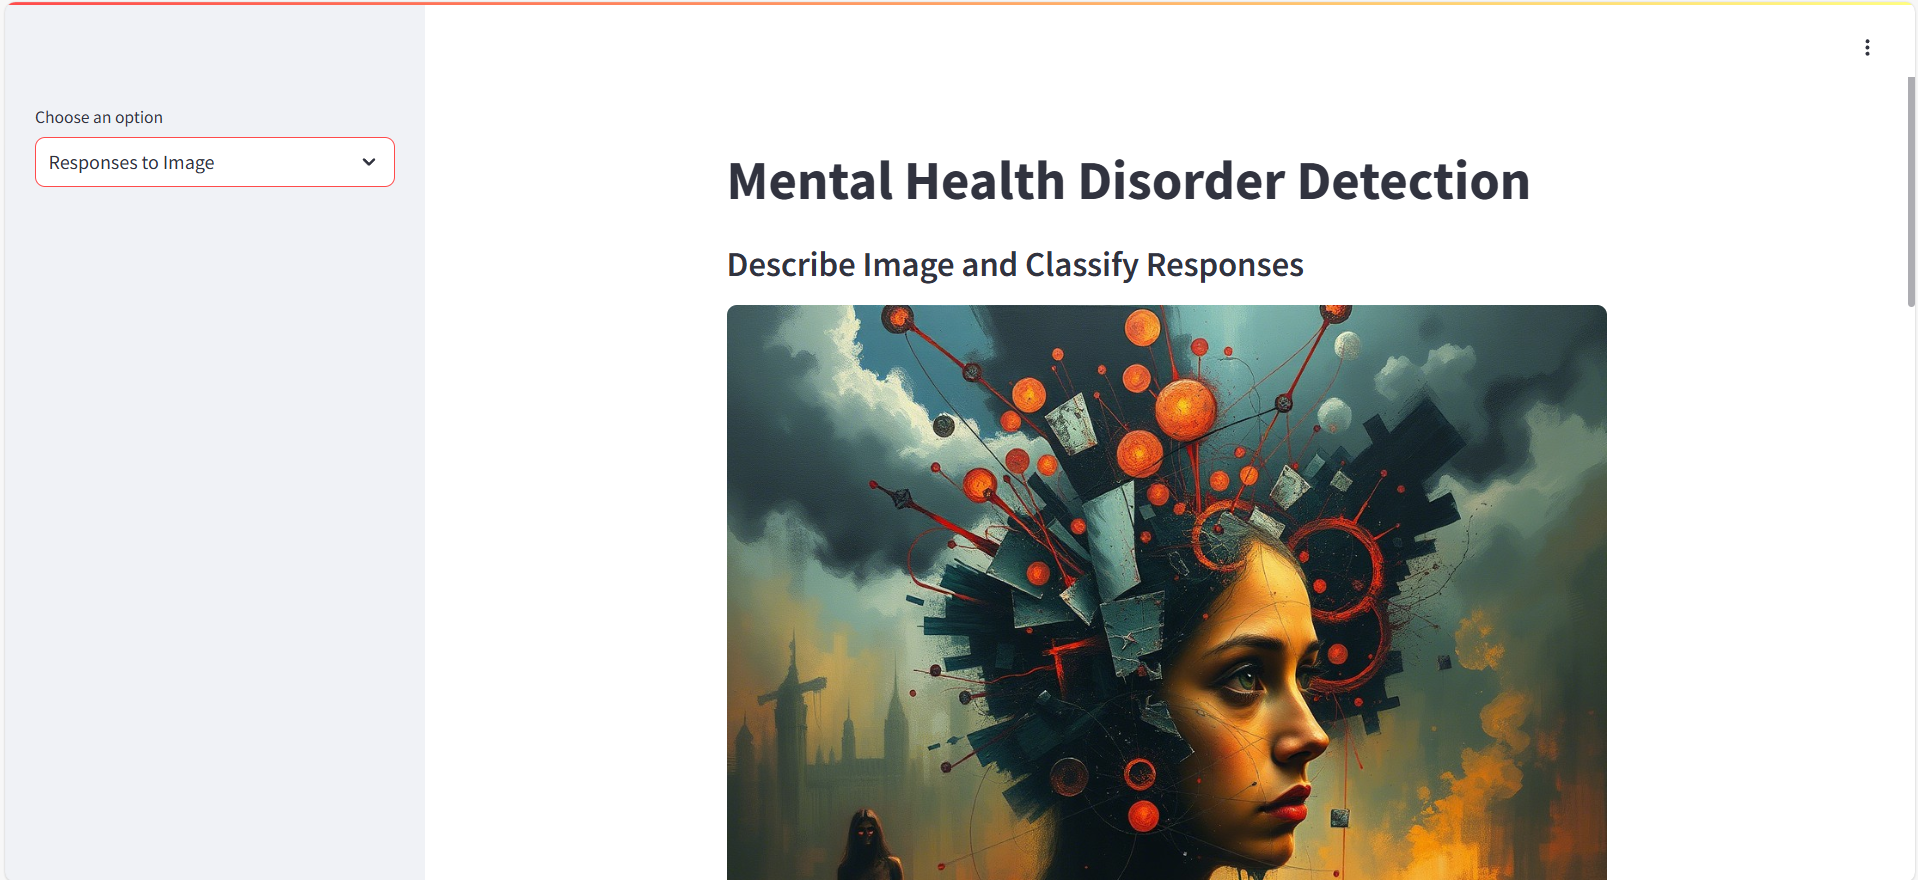
\includegraphics[width=\textwidth]{App Images/26 Interface.png}
        \caption*{User response to Image Option}
        \label{fig:26Interface}
    \end{subfigure}
    \hfill
    % Second subfigure: Questions related to image
    \begin{subfigure}[b]{0.495\textwidth}
        \centering
        \includegraphics[width=\textwidth]{App Images/27 Interface.png}
        \caption*{Questions related to image}
        \label{fig:27Interface}
    \end{subfigure}
    \label{fig:imageResponseAndQuestions}
\end{figure}

\vspace{-2em}

\begin{figure}[H]
    \centering
    % First subfigure: Reddit User Analysis
    \begin{subfigure}[b]{0.495\textwidth}
        \centering
        \includegraphics[width=\textwidth]{App Images/06 Interface.png}
        \caption*{Reddit User Analysis Option}
        \label{fig:07i}
    \end{subfigure}
    \hfill
    % Second subfigure: Twitter User Analysis
    \begin{subfigure}[b]{0.495\textwidth}
        \centering
        \includegraphics[width=\textwidth]{App Images/08 Interface.png}
        \caption*{Twitter User Analysis Option}
        \label{fig:09i}
    \end{subfigure}
    \label{fig:reddit_twitter_analysis}
\end{figure}

\pagebreak

\begin{figure}[h!]
    \centering
    % First subfigure: Prediction and Insights
    \begin{subfigure}[b]{0.495\textwidth}
        \centering
        \includegraphics[width=\textwidth]{App Images/03 Interface.png}
        \caption*{Prediction and Insights}
        \label{fig:03i}
    \end{subfigure}
    \hfill
    % Second subfigure: Social Media User Analysis
    \begin{subfigure}[b]{0.495\textwidth}
        \centering
        \includegraphics[width=\textwidth]{App Images/07 Interface.png}
        \caption*{Social Media User Analysis}
        \label{fig:08i}
    \end{subfigure}
    \label{fig:combined_analysis}
\end{figure}

\vspace{-2em}

\begin{figure}[h!]
    \centering
    % First subfigure: Model Retraining Result
    \begin{subfigure}[b]{0.495\textwidth}
        \centering
        \includegraphics[width=\textwidth]{App Images/17 Interface.png}
        \caption*{Model Retraining Result}
        \label{fig:10i}
    \end{subfigure}
    \hfill
    % Second subfigure: Emotion analysis
    \begin{subfigure}[b]{0.495\textwidth}
        \centering
        \includegraphics[width=\textwidth]{App Images/12-1 Interface.png}
        \caption*{Emotion analysis}
        \label{fig:10i23}
    \end{subfigure}
    \label{fig:comparison}
\end{figure}

\vspace{-2em}

\begin{figure}[h!]
    \centering
    % First subfigure: Generate Image Caption
    \begin{subfigure}[b]{0.495\textwidth}
        \centering
        \includegraphics[width=\textwidth]{App Images/18 Interface.png}
        \caption*{Generate Image Caption}
        \label{fig:10i234}
    \end{subfigure}
    \hfill
    % Second subfigure: Knowledge Graph after prediction
    \begin{subfigure}[b]{0.495\textwidth}
        \centering
        \includegraphics[width=\textwidth]{App Images/19 Interface.png}
        \caption*{Knowledge Graph after prediction}
        \label{fig:10i23445}
    \end{subfigure}
    \label{fig:generated_caption_vs_kg}
\end{figure}

\vspace{-2em}

\begin{figure}[H]
    \centering
    % First subfigure: Weighted Sum Analysis
    \begin{subfigure}[b]{0.495\textwidth}
        \centering
        \includegraphics[width=\textwidth]{App Images/22 Interface.png}
        \caption*{Weighted Sum Analysis}
        \label{fig:weighted_sum}
    \end{subfigure}
    \hfill
    % Second subfigure: Cosine Similarity Analysis
    \begin{subfigure}[b]{0.495\textwidth}
        \centering
        \includegraphics[width=\textwidth]{App Images/23 Interface.png}
        \caption*{Cosine Similarity Analysis}
        \label{fig:cosine_similarity}
    \end{subfigure}
    \label{fig:analysis_comparison}
\end{figure}

\pagebreak

\begin{figure}[h!]
    \centering
    % First subfigure: Euclidean Distance Analysis
    \begin{subfigure}[b]{0.495\textwidth}
        \centering
        \includegraphics[width=\textwidth]{App Images/24 Interface.png}
        \caption*{Euclidean Distance Analysis}
        \label{fig:euclidean_distance}
    \end{subfigure}
    \hfill
    % Second subfigure: Specific Parameter based Insights
    \begin{subfigure}[b]{0.495\textwidth}
        \centering
        \includegraphics[width=\textwidth]{App Images/25 Interface.png}
        \caption*{Specific Parameter based Insights}
        \label{fig:specific_insights}
    \end{subfigure}
    \label{fig:analysis_comparison}
\end{figure}

\vspace{-2em}

\begin{figure}[h!]
    \centering
    % First subfigure: Well-being survey questions
    \begin{subfigure}[b]{0.495\textwidth}
        \centering
        \includegraphics[width=\textwidth]{App Images/28 Interface.png}
        \caption*{Well-being survey option}
        \label{fig:wellbeing_questions}
    \end{subfigure}
    \hfill
    % Second subfigure: Well-being survey result
    \begin{subfigure}[b]{0.495\textwidth}
        \centering
        \includegraphics[width=\textwidth]{App Images/29 Interface.png}
        \caption*{Well-being survey questions}
        \label{fig:wellbeing_result}
    \end{subfigure}
    \label{fig:wellbeing_comparison}
\end{figure}

\vspace{-2em}

\begin{figure}[h!]
    \centering
    % First subfigure: Well-being survey questions
    \begin{subfigure}[b]{0.495\textwidth}
        \centering
        \includegraphics[width=\textwidth]{App Images/30 Interface.png}
        \caption*{Well-being survey result}
        \label{fig:wellbeing_questions}
    \end{subfigure}
    \hfill
    % Second subfigure: Well-being survey result
    \begin{subfigure}[b]{0.495\textwidth}
        \centering
        \includegraphics[width=\textwidth]{App Images/31 Interface.png}
        \caption*{Updated Association Matrix after responses}
        \label{fig:wellbeing_result}
    \end{subfigure}
    \label{fig:wellbeing_comparison}
\end{figure}

\vspace{-2em}

\begin{figure}[H]
    \centering
    % First subfigure: Well-being survey questions
    \begin{subfigure}[b]{0.495\textwidth}
        \centering
        \includegraphics[width=\textwidth]{App Images/34 Interface.png}
        \caption*{RAG based Wellbeing Insights}
        \label{fig:wellbeing_questions}
    \end{subfigure}
    \hfill
    % Second subfigure: Well-being survey result
    \begin{subfigure}[b]{0.495\textwidth}
        \centering
        \includegraphics[width=\textwidth]{App Images/35 Interface.png}
        \caption*{Match Visualization and Dataset Updation}
        \label{fig:wellbeing_result}
    \end{subfigure}
    \label{fig:wellbeing_comparison}
\end{figure}


\pagebreak
% ------------------------ Result and Analysis Ends -------------------------
